%%% Local Variables:
%%% mode: latex
%%% TeX-master: t
%%% End:
\chapter{弹性波模式解耦最小平方逆时偏移}
\label{cha:MD-ELSRTM}
\section{引言}
%前一章内容中我们将模型分解为高波数与中低波数成分,并通过弹性波WERTI方式来恢复模型的中低波数成分。
随着勘探目标的复杂化,传统偏移成像方法所获得的地下构造图像已经不能满足需求,人们希望获得振幅保真的地下反射率模型,来进而估计
介质参数、预测岩性等。
早期,基于Kirchhoff偏移的真振幅成像技术通过考虑不同偏移距(或入射角)的积分权重
来获得高保真的地下反射界面成像\cite{BeylkinEtAl1985,Bleistein1987}。
目前随着计算机技术的发展,RTM技术广泛应用于地震偏移成像中,真振幅的RTM成像方法也随之出现,例如
Zhang et al.
(2014)\cite{Zhang2014}给出了RTM框架下的振幅校正因子,目的是为速度和阻抗反演提供好的成像结果。

除了真振幅成像技术之外,最小平方偏移通过多次迭代来拟合观测与模拟的反射波数据以实现弹性参数高波数成分的重构。
受到计算能力的限制,早期的最小平方偏移也基于射线近似来实现(Schuster, 1993\cite{Schuster1993}; Nemeth
et al., 1999\cite{Nemeth1999})。
由于RTM能够应对复杂介质中射线理论难以处理的多路径问题,基于波动理论的最小平方逆时偏移(LSRTM)也逐渐成为近年来的研究热点。
它假设在已经获得足够好的速度模型中低波数成分之后恢复模型的高频扰动,
可视为线性的全波形反演。
%使得在最小平方意义下,
%用该“像”所预测的反射数据能与观测数据达到最佳匹配。因此,最小平方逆时偏移与全波形反演的理论框架是一致的。

%常规的FWI算法可以恢复模型的高波数成分,但是会受到许多因素干扰,
%如cycle-skipping问题,信噪比低,地震子波未知,正演算子不准确等等。除FWI之外,我们通常也会通过最小平方偏移(LSM)来实现高波数成分的重构。
%早在1993年,Schuster(1993)\cite{Schuster1993}提出了针对井间数据的LSM算法,而Nemeth et al.\cite{Nemeth1999}将该方法应用到了地面数据中。
%以波动方程为引擎的最小平方逆时偏移(LSRTM)近年来一直是研究的热点,例如Dai and
%Schuster(2013)\cite{Dai2013},Dong et al.(2012)\cite{Dong2012}, Luo and
%Hale(2014)\cite{Luo2014}。尽管其计算代价昂贵,但是LSRTM可以回避模型速度复杂时所产生的多路径问题。
%LSRTM的过程通常被认为是线性的全波形反演,其假设在已经获得足够好的低波数模型成分之后恢复模型的高频扰动,也即获得“像”,使得在最小平方意义下,
%用该“像”所预测的反射数据能与观测数据达到最佳匹配。因此,最小平方逆时偏移与全波形反演的理论框架是一致的。

%通过考虑不同模型参数到正演方程中,LSRTM可在反演过程中获得不同参数的高频扰动。
为了更准确地描述波传播过程,同时获得更多的参数
扰动,许多学者发展了多参数的LSRTM方法,
例如Yang et
al.(2016)\cite{Yang2016}通过散射积分法,利用Hessian信息约束变密度声波介质中的LSRTM以获得速度与密度的高频扰动。
近期,恢复弹性介质中的高频参数扰动获得了高度关注。
例如,Duan et al. (2016)\cite{Duan2016}, Feng and Schuster(2016)\cite{Feng2016}和Xu et al.(2016)
\cite{Xu2016}几乎同时发展了ELSRTM方法,Ren et al. (2016)\cite{RenEtAl2016}重点调查了不同目标函数对ELSRTM的影响。
相比声波成像,弹性波成像可以提供更多的地下信息同时也存在更复杂的问题,
例如成像中不同波模式产生的“cross-talk”假象、PS波成像中的极性反转问题以及如何选取合适的成像条件获取更具有物理意义的成像结果等等(Du et al,
2014\cite{DuEtAl2014}; Wang et al.,
2016\cite{wang2016scalar}; Gong et
al, 2016\cite{GongEtAl2016};Rocha et al,2016\cite{RochaEtAl2016a})。

最近,从反演理论框架出发,已有学者(
如Duan et al.(2016)\cite{Duan2016},Feng et
al.(2016)\cite{Feng2016})
推导出了与EFWI梯度非常类似的成像公式。本质上获得的是高频的参数扰动对应的梯度,同时回避了常规成像条件下的极性反转问题。
本章从矩阵形式的位移-应力弹性波方程出发,给出了类似的梯度公式,并引入模式解耦对ELSRTM进行梯度预条件。
根据参数模型不同的耦合程度,设计相应的反演策略并测试其在ELSRTM中压制参数耦合效应的效果。
%而基于
%第二章中对EFWI算法的分析,模式解耦带来的优势将同样能在ELSRTM中得以应用,因此我们将在本章中应用波模式解耦来对ELSRTM进行预条件,从而获得更好结果。
\section{矩阵形式的弹性波方程}
与第二章类似,将从弹性波方程出发推导ELSRTM目标函数关于弹性参数高波数扰动的梯度。为了方便,同样在频率域
利用矩阵形式的弹性波方程来完成推导。时空域二维位移-应力弹性波方程为:
\begin{equation}
\begin{split}
   & \rho\frac{\partial^2 u_{x}}{\partial t^2}=	\frac{\partial \tau_{xx}}{\partial x}+
		\frac{\partial \tau_{xz}}{\partial z},\\
   & \rho\frac{\partial^2 u_{z}}{\partial t^2}=	\frac{\partial \tau_{xz}}{\partial x}+
		\frac{\partial \tau_{zz}}{\partial z},\\
   & \tau_{xx}=(\lambda+2\mu)\frac{\partial u_x}{\partial x}+\lambda\frac{\partial u_z}{\partial z},\\
   & \tau_{zz}=\lambda\frac{\partial u_x}{\partial x}+(\lambda+2\mu)\frac{\partial u_z}{\partial z},\\
   & \tau_{xz}=\mu(\frac{\partial u_x}{\partial z} + \frac{\partial u_z}{\partial x}),
    \label{eq:WE_LSRTM}
\end{split}
\end{equation}
方程\eqref{eq:WE_LSRTM}可以改写为频率域形式:
\begin{equation}
\mathbf{L}(\lambda,\mu,\rho)\mathbf{U}=\mathbf{f},
    \label{eq:WE_Matrix} 
\end{equation}
其中位移场与应力场构成的波场矢量满足$\mathbf{U}=[u_x,u_z,\tau_{xx},\tau_{zz},\tau_{xz}]^T$,$\mathbf{f}$为震源,并且算子矩阵$\mathbf{L}$满足:
\begin{equation}
        \mathbf{L}
        =
        \begin{bmatrix}
%			&\rho\partial^2_{tt} &0 &-\partial_x & 0 &-\partial_z\\
			&-\rho\omega^2 &0 &-\partial_x & 0 &-\partial_z\\
			& 0  &-\rho\omega^2 &0 &-\partial_z &-\partial_x\\
%			& 0  &\rho\partial^2_{tt} &0 &-\partial_z &-\partial_x\\
			&-(\lambda+2\mu)\partial_x &-\lambda\partial_z &1 &0&0\\
			& -\lambda\partial_x  &-(\lambda+2\mu)\partial_z &0 &1&0\\
			& -\mu\partial_z  &-\mu\partial_x &0 &0&1\\
        \end{bmatrix},
        \label{eq:L}
\end{equation}
上式中$\omega$为角频率,$\partial_x$和$\partial_z$分别代表模型空间中沿x和z方向的一阶导数,假设$\rho,\lambda,\mu$为弹性介质背景参数,当存在模型扰动
$\delta\lambda,\delta\mu,\delta\rho$时,介质中总波场($\mathbf{U}+\delta
\mathbf{U}$)和扰动场($\delta \mathbf{U}$)满足:
\begin{equation}
\mathbf{L}(\lambda+\delta\lambda,\mu+\delta\mu,\rho+\delta\rho)(\mathbf{U+\delta U})=\mathbf{f},
    \label{eq:WE_Matrix_all} 
\end{equation}
将式\eqref{eq:WE_Matrix_all}减去式\eqref{eq:WE_Matrix}则可得Born近似下扰动波场$\delta
\mathbf{U}$与背景波场$\mathbf{U}$之间的关系:
\begin{equation}
\mathbf{L}(\lambda,\mu,\rho)\mathbf{\delta U}=\mathbf{L}^{'}\mathbf{U},
    \label{eq:WE_Matrix_delta} 
\end{equation}
其中$\mathbf{L}^{'}=(\delta\lambda\mathbf{L}^{'}_{\lambda}+\delta\mu\mathbf{L}^{'}_{\mu}+\delta\rho\mathbf{L}^{'}_{\rho})$,且
\begin{equation}
        \mathbf{L}^{'}_{\lambda}=
        \begin{bmatrix}
			&0 &0 &0 & 0 &0\\
			& 0  &0 &0 &0 &0\\
			&\partial_x &\partial_z &0 &0&0\\
			& \partial_x  &\partial_z &0 &0&0\\
			& 0  &0&0 &0&0\\
        \end{bmatrix},
%        \label{eq:L_lambda}
        \mathbf{L}^{'}_{\mu}=
        \begin{bmatrix}
            &0 &0 &0 & 0 &0\\
            & 0  &0 &0 &0 &0\\
            &2\partial_x &0 &0 &0&0\\
            & 0  &2\partial_z &0 &0&0\\
            & \partial_z  &\partial_x&0 &0&0\\
        \end{bmatrix},
        \label{eq:L_lambdamu}
\end{equation}
\begin{equation}
        \mathbf{L}^{'}_{\rho}=
        \begin{bmatrix}
		&\omega^2 &0 &0 & 0 &0\\
            & 0  &\omega^2 &0 &0 &0\\
            &0&0 &0 &0&0\\
            &0  &0 &0 &0&0\\
            & 0  &0&0 &0&0\\
        \end{bmatrix}.
        \label{eq:L_rho}
\end{equation}
ELSRTM通常假设背景模型及背景波场不发生变化。%故可将方程\eqref{eq:WE_Matrix_delta}看作为新的状态方程。
与EFWI中所描述的正问题不同的是,方程\eqref{eq:WE_Matrix_delta}所描述的正问题只考虑反射(散射)波而不包含透射波(或直达波)。
方程右端项为背景波场与参数扰动之间相互作用形成的次级源。
上述问题通常假定在背景弹性参数模型足够好的时候来恢复高波数扰动,因此方程也只描述单次散射过程。
实际地下介质中的多次散射效应会对成像带来影响。近期,也有学者考虑在反演迭代过程中将更新的扰动量加入背景场。
例如,Guo and
Alkhalifah(2016)\cite{Guo2016}所展示的RWI过程中,他们将界面扰动引起的散射场加入到背景场中以便一定程度上考虑多次散射效应的影响。
\section{弹性波最小平方逆时偏移}
本文ELSRTM中同样利用$L_2$范数来定义目标函数:
\begin{equation}
    E=\frac{1}{2}\sum_{\omega}\sum_{s,r}\left\lVert \mathfrak{F}\delta \mathbf{U}-\mathbf{d}^{obs} \right \rVert^2,
    \label{eq:misfit_LSRTM}
\end{equation}
其中$\mathfrak{F}$为采样函数,$\delta\mathbf{U}$为模拟的反射波数据,$s,r$代表炮点和检波点位置
。该目标函数要对所有频率、所有炮检对的反射数据残差求和。利用拉格朗日乘子法,建立增广函数:
\begin{equation}
\begin{split}
    \mathcal{L}(\delta\mathbf{U},\bm\Psi,\delta\lambda,\delta\mu,\delta\rho)=&Re\left[
	\frac{1}{2}\sum_{\omega}\sum_{s,r}\left\lVert \mathfrak{F}\delta \mathbf{U}-\mathbf{d}^{obs} \right \rVert^2 \right. \\
	&\left.-\sum_{\omega}\sum_{s}\langle\bm\Psi,\mathbf{L}\delta\mathbf{U}-\mathbf{L}^{'}\mathbf{U}\rangle_{\mathbf{x}}\right],
    \label{eq:Lagrangian_LSRTM}
\end{split}
\end{equation}
这里$\bm\Psi=(\hat {u}_x,\hat {u}_z,\hat{\tau}_{xx},\hat{\tau}_{zz},\hat{\tau}_{xz})^T$为伴随波场,$\langle\cdot\rangle_\mathbf{x}$
代表空间域的内积运算,根据Plessix(2006)\cite{plessix2006},该优化问题的极值点需要满足
$\frac{\partial\mathcal{L}}{\partial(\delta\mathbf{U})}=0$,于是得到伴随状态方程:
\begin{equation}
	\mathbf{L}^*(\lambda,\mu,\rho)\bm\Psi_s=\sum_{r}(\mathfrak{F}\delta\mathbf{U}-\mathbf{d}^{obs}),
    \label{eq:Adjoint_LSRTM} 
\end{equation}
$\mathbf{L}^*$为正传算子$\mathbf{L}$的共轭转置,代表了传播算子的逆时反传。
右端项则代表了每炮数据检波点处的残差波场。
因此,伴随波场$\bm\Psi$是以数据残差为震源的逆时
传播波场。
由于每一炮每一个频率的数据都对应一个共轭方程,因此上式中未出现对频率及炮点的求和。为了简单起见,隐去式\eqref{eq:Adjoint_LSRTM}中的采样函数。
于是,式\eqref{eq:Lagrangian_LSRTM}对应的梯度应为:
\begin{equation}
    \frac{\partial\mathcal{L}}{\partial \delta\mathbf{m}}=Re\left(\sum_{\omega}\sum_{s,r}
	\langle\bm\Psi,\frac{\partial
		\mathbf{L}^{'}}{\partial\delta\mathbf{m}}\mathbf{U}\rangle_{\mathbf{x}}\right),
    \label{eq:Gradient_LSRTM}
\end{equation}
其中$\delta\mathbf{m}=(\delta\lambda, \delta\mu,\delta\rho)$,
注意到$\frac{\partial\mathcal{L}}{\partial \delta\mathbf{m}}$的有关导数包括$\frac{\partial\mathcal{L}}{\partial 
\delta\lambda}=\mathcal{L}^{'}_{\lambda}$,$\frac{\partial\mathcal{L}}{\partial\delta\mu}=\mathcal{L}^{'}_{\mu}$以及
$\frac{\partial\mathcal{L}}{\partial\delta\rho}=\mathcal{L}^{'}_{\rho}$。
利用式\eqref{eq:L_lambdamu}-\eqref{eq:L_rho}对$\delta\mathbf{m}$求导并将其转换到时间域,
可得:
\begin{equation}
\begin{split}
   & \frac{\partial\mathcal{L}}{\partial \delta\lambda}=\sum_{s,r}\int^T_{0}
	(\frac{\partial u_x}{\partial x}+\frac{\partial u_z}{\partial z})(\hat{\tau}_{xx}+\hat{\tau}_{zz}),\\
   & \frac{\partial\mathcal{L}}{\partial \delta\mu}=\sum_{s,r}\int^T_{0}
	2(\frac{\partial u_x}{\partial x}\hat{\tau}_{xx}+\frac{\partial u_z}{\partial z}\hat{\tau}_{zz})+
	(\frac{\partial u_x}{\partial z}+\frac{\partial u_x}{\partial z})\hat{\tau}_{xz},\\
   & \frac{\partial\mathcal{L}}{\partial \delta\rho}=-\sum_{s,r}\int^T_{0}
   \frac{\partial^2 u_x}{\partial t^2}\hat{u}_x+\frac{\partial^2 u_z}{\partial t^2}\hat{u}_{z}.
    \label{eq:Gradient_lambdamurho_LSRTM}
\end{split}
\end{equation}
%可以看到上式中梯度的表达式与EFWI中的表达(式\ref{eq:DeGradient_vpvsrho})几乎一致,只是参与相关的波场分量不同。这也说明ELSRTM与EFWI之间密不可分
%的关系。

另外需要注意的是,将式\eqref{eq:Adjoint_LSRTM}变换到时空域并展开,可得:
\begin{equation}
\begin{split}
	& \rho\frac{\partial^2 \hat{u}_{x}}{\partial t^2}=	\frac{\partial (\lambda+2\mu)\hat{\tau}_{xx}}{\partial x}+
		\frac{\partial \lambda\hat{\tau}_{zz}}{\partial x}+\frac{\partial \mu
			\hat{\tau}_{xz}}{\partial z}+\delta d_x,\\
		& \rho\frac{\partial^2 \hat{u}_{z}}{\partial t^2}=	\frac{\partial \lambda\hat{\tau}_{xx}}{\partial z}+
		\frac{\partial (\lambda+2\mu)\hat{\tau}_{zz}}{\partial z}+\frac{\partial \mu
			\hat{\tau}_{xz}}{\partial x}+\delta d_z,\\
		& \hat{\tau}_{xx}=\frac{\partial \hat{u}_x}{\partial x}, \hat{\tau}_{zz}=\frac{\partial \hat{u}_z}{\partial z},\\
		& \hat{\tau}_{xz}=\frac{\partial \hat{u}_x}{\partial z} + \frac{\partial \hat{u}_z}{\partial x}.
    \label{eq:Time_Adjoint_WE_LSRTM}
\end{split}
\end{equation}
其中$\delta \mathbf{d}=\mathfrak{F}\delta\mathbf{U}-\mathbf{d}^{obs}$.
可见在反传波场的求取过程中,由于共轭转置算子的作用导致伴随状态方程与原本的弹性波方程形式不同,新的方程中多出了两项应力导数项。
伴随波场的应力应变关系也发生了改变,这是求解中需要注意的。
%但是我们也通过实验发现,采用新的方程也并未带来非常大的不同,可以说新方程在数学导出上不一样,但是
%不影响物理过程。
\section{模式解耦梯度预条件}
可以看到ELSRTM梯度表达式与EFWI中的梯度(式\ref{eq:DeGradient_vpvsrho})非常类似,只是后者中$\lambda$和$\mu$的梯度计算涉及的波场都是位移的空间导数,而
前者梯度中采用到位移场空间导数与应力场,密度的梯度表达式则完全一致。
采用速度-密度的参数化方式,可以导出目标函数关于$V_p$与$V_s$的梯度:
\begin{equation}
\begin{split}
   & \frac{\partial\mathcal{L}}{\partial \delta V_p}=2\rho V_p\frac{\partial\mathcal{L}}{\partial \delta \lambda}\\
   & \frac{\partial\mathcal{L}}{\partial \delta V_s}=2\rho V_s(-2\frac{\partial\mathcal{L}}{\partial \delta \lambda}
	+\frac{\partial\mathcal{L}}{\partial \delta \mu})\\
   & \frac{\partial\mathcal{L}}{\partial \delta\rho_{vel}}=(V^2_p-2V^2_s)\frac{\partial\mathcal{L}}{\partial \delta \lambda}+V^2_s\frac{\partial\mathcal{L}}{\partial \delta \lambda}+\frac{\partial\mathcal{L}}{\partial \delta\rho}.
    \label{eq:Gradient_VpVsrho_LSRTM}
\end{split}
\end{equation}

为了利用模式解耦来降低$V_p$和$V_s$之间的trade-off,同样在ELSRTM中暂不考虑密度扰动。
于是,考虑模式解耦的梯度为:
\begin{equation}
\begin{split}
   & \frac{\partial\mathcal{L}}{\partial \delta V_p}=2\rho V_p\sum_{s,r}\int^T_{0}
	(\frac{\partial u_x}{\partial x}+\frac{\partial u_z}{\partial
	z})(\hat{\tau}_{xx}+\hat{\tau}_{zz})dt,\\
   & \frac{\partial\mathcal{L}}{\partial \delta V_s}=2\rho V_s\sum_{s,r}\int^T_{0}
	2(\frac{\partial u_x}{\partial x}\hat{\tau}^S_{xx}+\frac{\partial u_z}{\partial z}\hat{\tau}^S_{zz})+
	(\frac{\partial u_x}{\partial z}+\frac{\partial u_x}{\partial
	z})\hat{\tau}^S_{xz}dt.
%   & \frac{\partial\mathcal{L}}{\partial \delta V_s}=-2\rho V_s\sum_{s,r}\int^T_{0}
%	2(\frac{\partial u^M_x}{\partial x}\hat{\tau}^S_{xx}+\frac{\partial u^M_z}{\partial z}\hat{\tau}^S_{zz})+
%	(\frac{\partial u^M_x}{\partial z}+\frac{\partial u^M_x}{\partial
%	z})\hat{\tau}^S_{xz}dt,
    \label{eq:Gradient_Vel_LSRTM}
\end{split}
\end{equation}
%其中$M\in{\{P,S\}}$。
注意,与EFWI所不同的是LSRTM假设已经获得了可靠的背景速度模型,只需要反演模型的高波数分量,因此所处理的数据频带一般较宽。但是,
在高频数据中,当介质模型复杂时,层间多次波或者多次散射也会比较严重。尤其是在利用S波数据进行LSRTM的情况下,S波波场本身能量较弱,
在S波多次散射或者转换严重的区域会对解耦之后的梯度产生很不利的干扰。
%因此,对正传波场的解耦可能也会有助于减少假象与干扰。
这一点与第二章EFWI不太一样,因为EFWI通常不会牵涉较高的频率成分,多次散射效应并不突出。
%所以是否解耦正传波场需要视情况而定。
%如果多次散射较弱,那么不用解耦正传波场,
%如果多次散射严重,就解耦正传波场用更多计算量来压制假象。

此外,前文也提到需要对梯度进行其他预条件才能更好的加速收敛,这里采用震源波场的能量来进行照明补偿:
\begin{equation}
	\mathbf{Q} =\left[\int^T_0(u^2_x+u^2_z)dt\right]^{-1},
    \label{eq:Gradient_Illumination_LSRTM}
\end{equation}
这里$\mathbf{Q}$相当于Hessian逆矩阵对角线元素的补偿作用。于是最终ELSRTM中高频参数扰动量的更新方式如下:
\begin{equation}
	\delta\mathbf{m}_{k+1}=\delta\mathbf{m}_{k}-\alpha_{k}
        \begin{bmatrix}\mathbf{Q}{\frac{\partial\mathcal{L}}{\partial \delta V_p}}\\
		\mathbf{Q}{\frac{\partial\mathcal{L}}{\partial \delta V_s}}\end{bmatrix}_{k},
        \label{eq:Gradientmethod_LSRTM}
\end{equation}
其中$\delta\mathbf{m}_{k}$为$k$次迭代的模型扰动,$\alpha$为k次迭代的步长。
步长搜索同样采用抛物线拟合的方式来求取。
\section{数值实验}
本节将通过数值实验来验证模式解耦在最小平方偏移中的功效。
由于ELSRTM第一次迭代与ERTM过程类似,因此除非特别说明,本节中所指ERTM都是ELSRTM首次迭代的结果。
将从简单模型出发分析ELSRTM中可能存在的问题,并在Marmousi-II模型上测试解耦预条件的ELSRTM算法与反演策略。
根据第二章中的分析结果,采用S波来反演$V_s$扰动接近于单参数的反演。ELSRTM为线性问题,
只需要更新模型高频扰动部分,因此在反演策略上也与EFWI略有不同。将根据不同的情况采取如下两种不同的反演策略:

策略1:$\delta V_p$较少受到耦合效应影响时,采用$\delta V_p$与$\delta
V_s$同时反演,并用模式解耦梯度预条件来压制参数耦合;

策略2:$\delta V_p$与$\delta V_s$耦合效应强烈时,先采用模式解耦梯度预条件对$\delta V_s$进行反演,在$\delta
V_s$反演得足够好的后再对$\delta V_p$进行反演。

策略1通过一次迭代获得双参数反演的结果,而策略2需要多耗费一轮迭代的计算量。
策略2中,先反演出合理的$\delta V_s$,这样数据中来自$\delta
V_s$的P波能量就会首先得到匹配,之后再反演$\delta
V_p$时这一部分P波残差就不会在梯度中产生太多的串扰,从而达到压制参数耦合的效果。需要注意的是,这一思路在EFWI中并不十分适用。
因为在EFWI中,需要
逐步地更新$V_p$模型的中低波数成分来确保
PS波数据的匹配不会陷入局部极值。与此同时,又要采用PS波数据以解耦的方式更新$V_s$使得P波残差较好地收敛以改善$V_p$的反演精度。
因此EFWI中更适合采用双参数同时反演来降低非线性程度。


\subsection{反射数据与Born模拟数据的差异}
LSRTM的理论是基于一阶Born散射导出的,因此由高频参数扰动预测的反射波其实是Born散射数据。所以在进行数据匹配的时候观测数据需要尽可能地接近Born散射数据
,才能保证数据残差的最佳拟合。事实上,采用Born模拟数据进行ELSRTM就是一种线性反散射求解。
而实际中无法获得Born散射数据,通常在进行LSRTM时都是匹配切除直达波的反射数据。由于实际反射数据与Born模拟数据之间存在差异,
如果反演时直接采用反射数据就会使得正演数据无法与观测数据完全匹配。

这里,用简单的两层介质来调查实际反射数据与Born模拟反射数据间的差异。这里只考虑$V_p$的扰动界面,
上层$V_p=2.6km/s$,下层$V_p=2.8km/s$, $V_s$采用均匀模型($V_s=1.5km/s$)。所用的有限差分算法空间采样10m,时间采样1ms。
由于Born近似在小扰动下成立,因此对真实模型进行不同尺度平滑后进行Born正演,以调查由弹性波方程直接计算出的反射数据与Born模拟数
据之间的差异。
\begin{figure}[!htb]
   \centering
   \subfloat[]{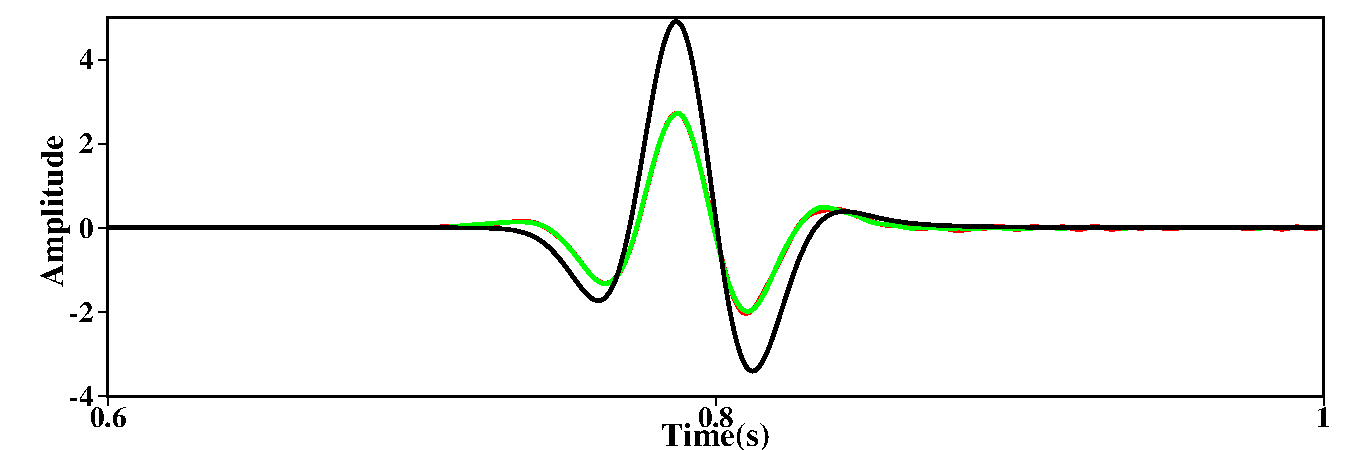
\includegraphics[width=0.8\textwidth]{Figure/chapter04/singlelayer/smooth3.pdf}}\\
   \subfloat[]{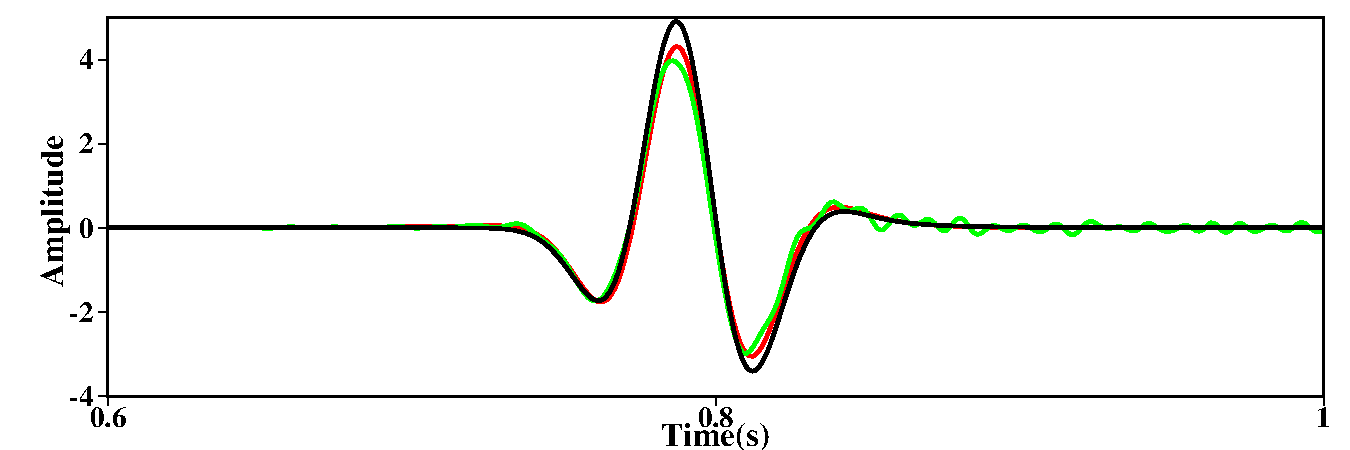
\includegraphics[width=0.8\textwidth]{Figure/chapter04/singlelayer/smooth8.pdf}}
   \caption{反射数据(黑)、剩余反射数据(红)和Born模拟数据(绿)之间的差异。(a)
   模型平滑窗口30m; (b)模型平滑窗口100m.}
   \label{fig:refl_born_comparison}
\end{figure}
\begin{figure}[!htb]
   \centering
   \subfloat{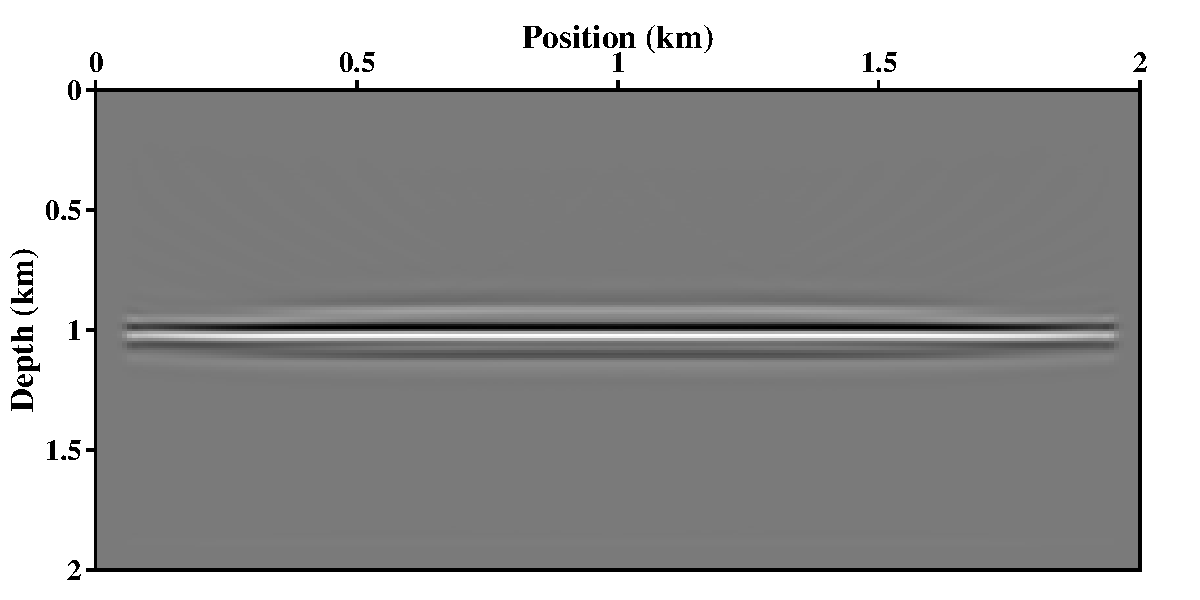
\includegraphics[width=0.5\textwidth]{Figure/chapter04/singlelayer/ref.pdf}
				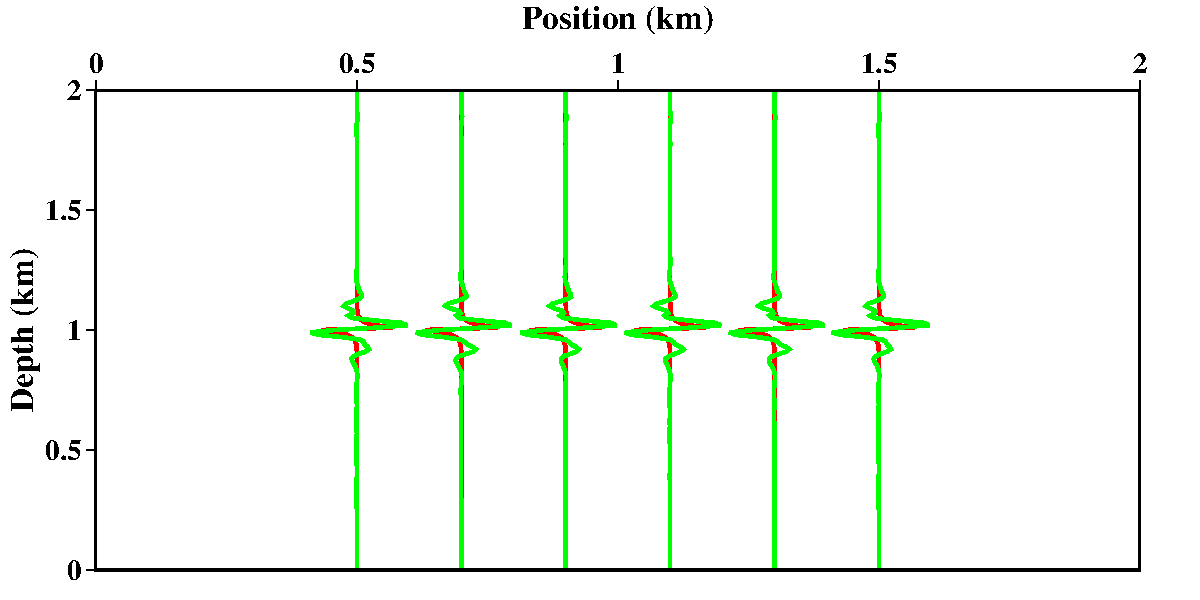
\includegraphics[width=0.5\textwidth]{Figure/chapter04/singlelayer/comparison1.pdf}}\\
   \subfloat{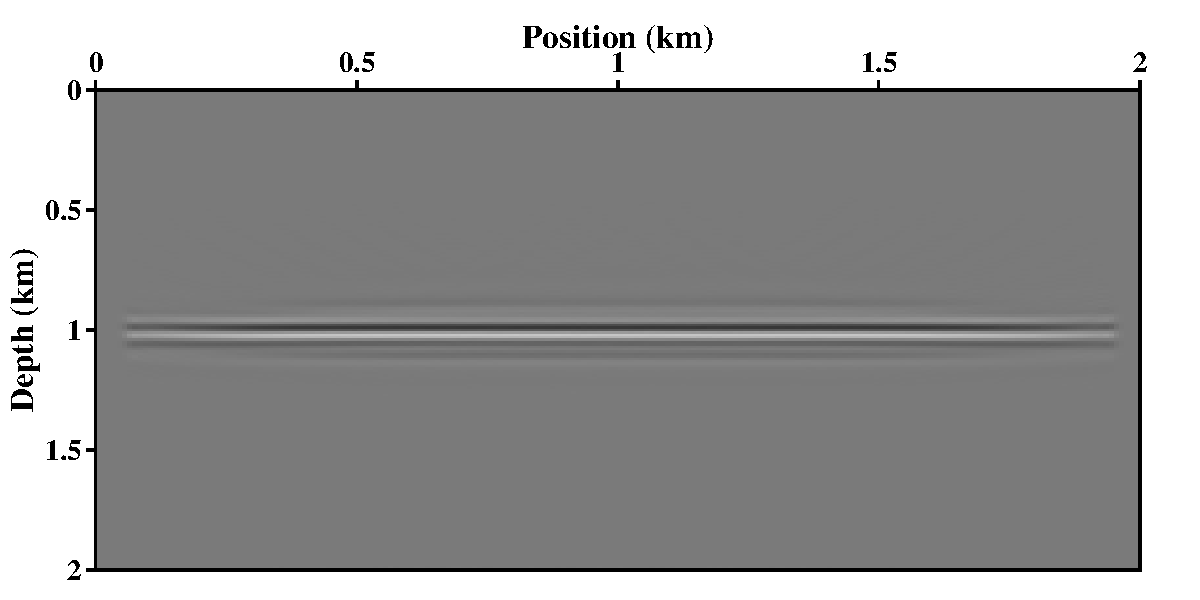
\includegraphics[width=0.5\textwidth]{Figure/chapter04/singlelayer/born.pdf}
			   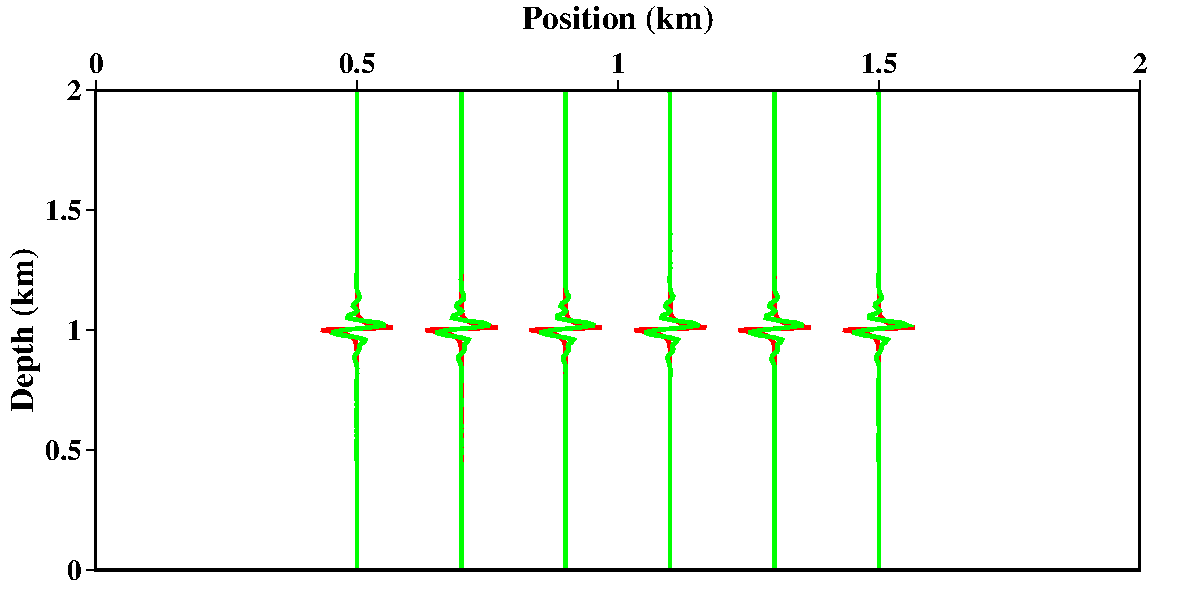
\includegraphics[width=0.5\textwidth]{Figure/chapter04/singlelayer/comparison2.pdf}}
%   \subfloat{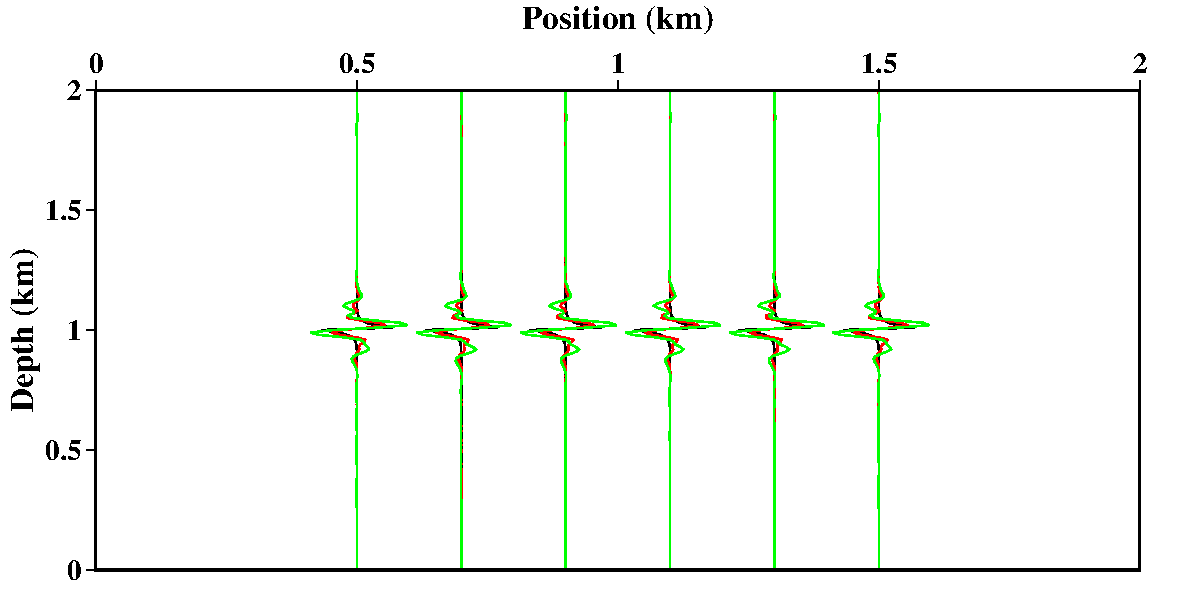
\includegraphics[width=0.5\textwidth]{Figure/chapter04/singlelayer/comparison.pdf}}
   \caption{图中左侧为ELSRTM的$\delta
	   V_p$,右侧为相应位置上的抽线对比。顶部为原始反射数据反演结果,底部为Born模拟数据反演结果。其中绿色代表反演结果,红色代表模型真实扰动。}
   \label{fig:Vpcomparison}
\end{figure}

图\ref{fig:refl_born_comparison}a为将真实模型按照30m半径平滑后正演所获得的反射数据、剩余反射数据(即
真实反射数据与背景波场记录的残差)
以及真实扰动产生的Born模拟数据三者之间的比较。可以看到,当平滑半径较小时,背景模型中会包含部分高波数成分,这就使得背景场中含有
部分反射能量,从而导致Born模拟数据与真实反射数据相差较远。在此模型中,由于反射数据振幅大于Born模拟数据的振幅,如果在反演中直接匹配该反射数据,
最终会导致反演中数据残差收敛时产生参数扰动的过估计(图\ref{fig:Vpcomparison})。
而如图\ref{fig:refl_born_comparison}b所示,剩余反射数据则可以与Born模拟数据很好地匹配,基于此来反演就可以避免产生过估计。

也就是说,如果模型中包含较强的反射能量时就需要匹配剩余反射数据,而不是反射数据本身。
如果模型平滑尺度较大,背景波场中包含的反射能量较弱,那么Born模拟数据将与反射数据
比较接近。但即便如此,Born模拟数据与反射数据之间的差异也大于它与剩余反射数据之间的差异
(图\ref{fig:refl_born_comparison}b)。因此在LSRTM时,匹配剩余反射数据
将是一个更好的选择。
\subsection{参数耦合分析}
\begin{figure}[!htb]
   \centering
   \subfloat[]{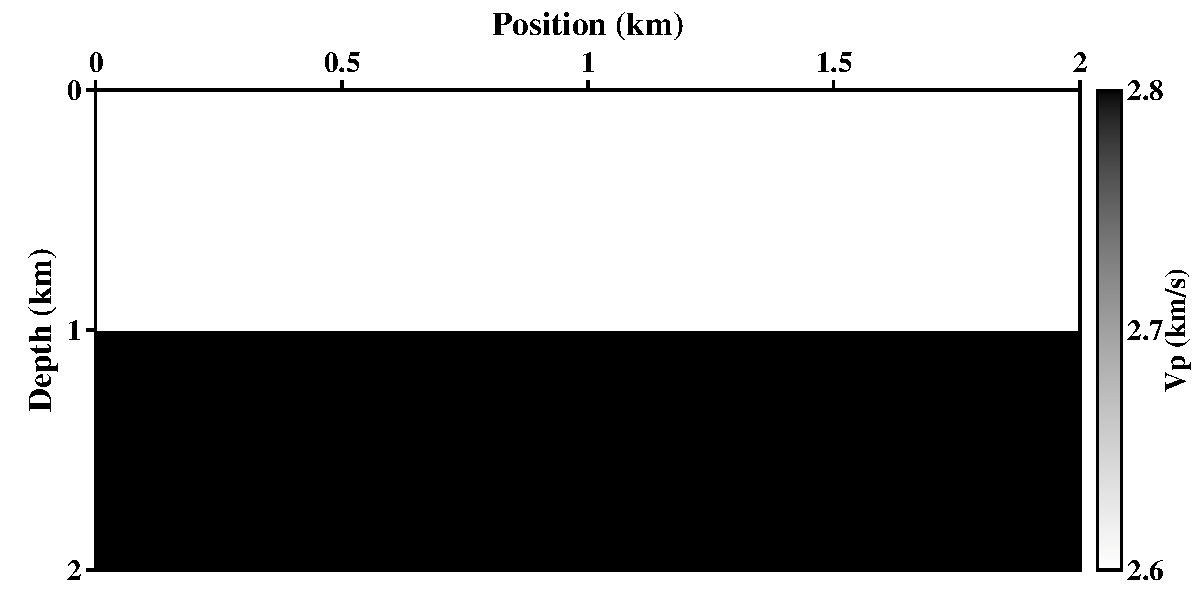
\includegraphics[width=0.5\textwidth]{Figure/chapter04/tradeoff/vp.pdf}}
   \subfloat[]{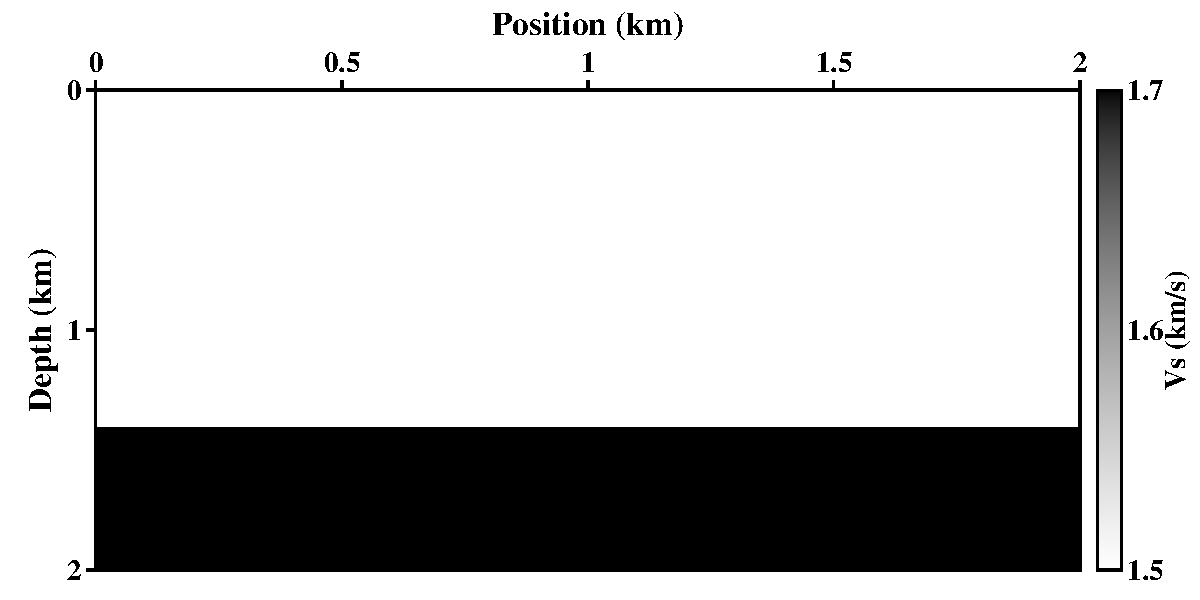
\includegraphics[width=0.5\textwidth]{Figure/chapter04/tradeoff/vs.pdf}}\\
   \caption{参数耦合测试真实模型: (a) $V_p$, (b) $V_s$.}
   \label{fig:tradeoffModel}
\end{figure}
\begin{figure}[!htb]
   \centering
   \subfloat[]{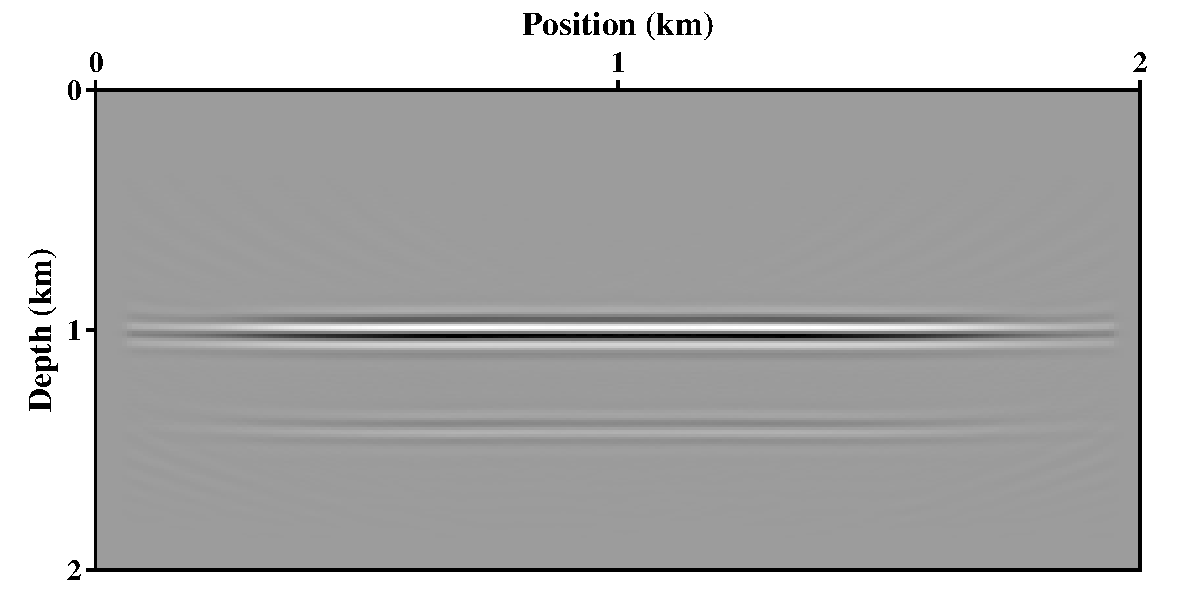
\includegraphics[width=0.5\textwidth]{Figure/chapter04/tradeoff/RTMvpnodecomp.pdf}}
   \subfloat[]{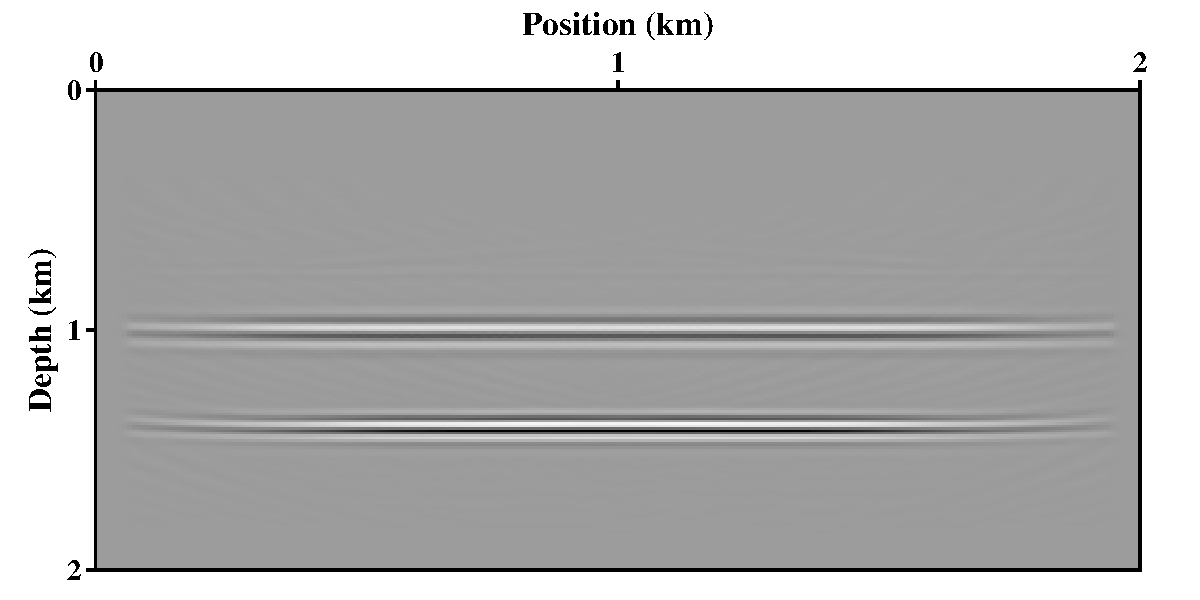
\includegraphics[width=0.5\textwidth]{Figure/chapter04/tradeoff/RTMvsnodecomp.pdf}}\\
   \subfloat[]{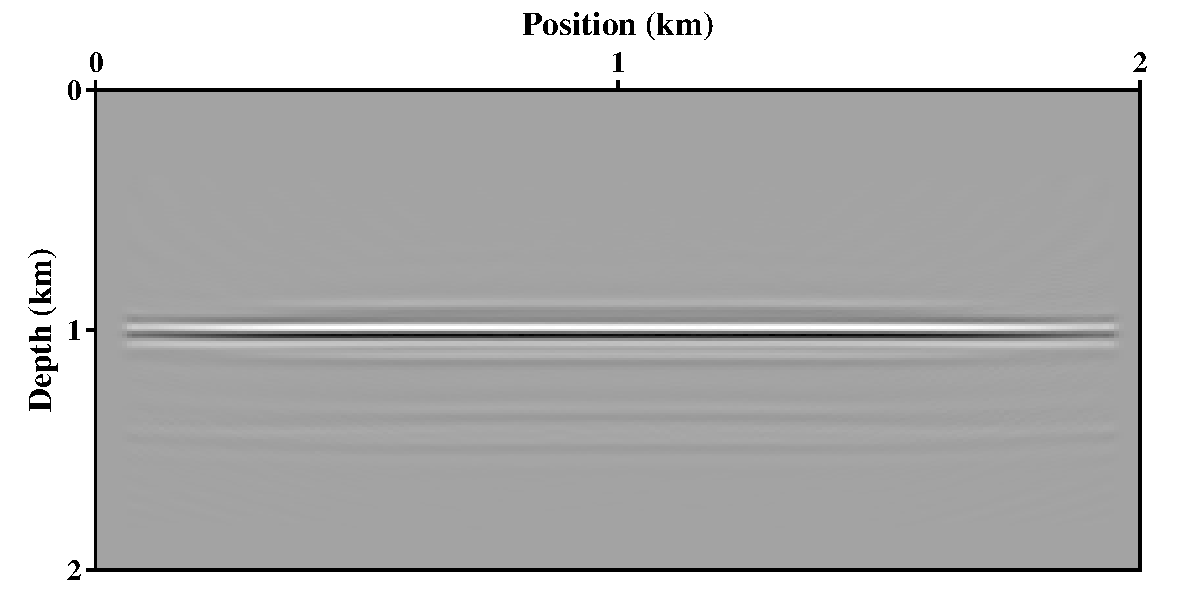
\includegraphics[width=0.5\textwidth]{Figure/chapter04/tradeoff/vpnodecomp.pdf}}
   \subfloat[]{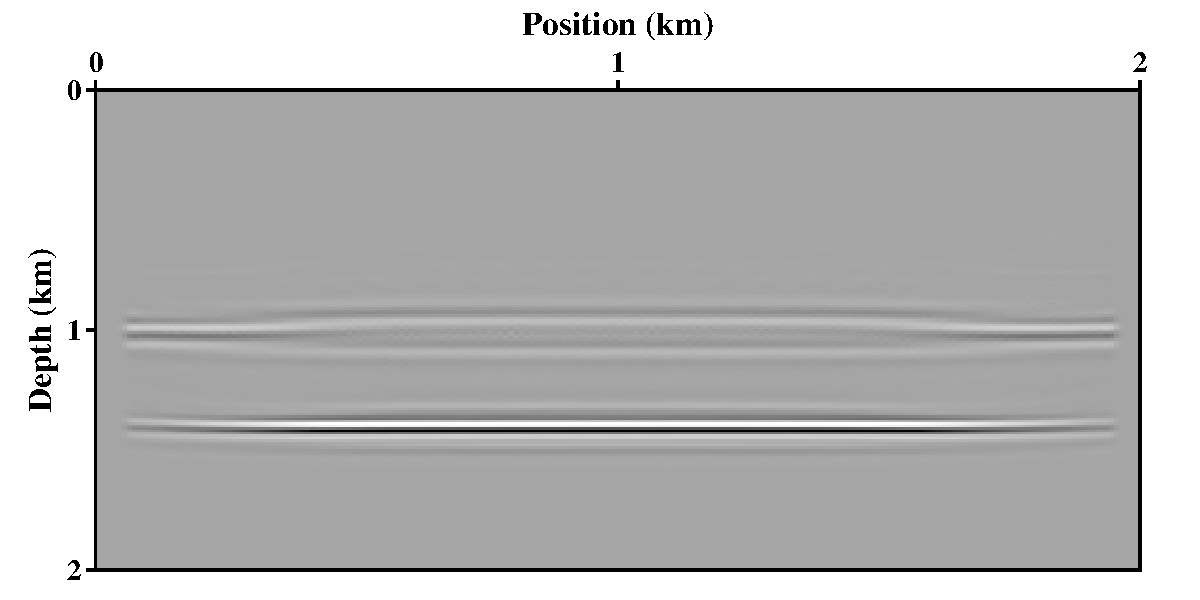
\includegraphics[width=0.5\textwidth]{Figure/chapter04/tradeoff/vsnodecomp.pdf}}
   \caption{常规ERTM与ELSRTM结果:左侧为$\delta V_p$,右侧为$\delta V_s$。(a), (b) ERTM结果;(c),
   (d) ELSRTM结果。}
   \label{fig:tradeoff_nodecomp}
\end{figure}
\begin{figure}[!htb]
   \centering
   \subfloat[]{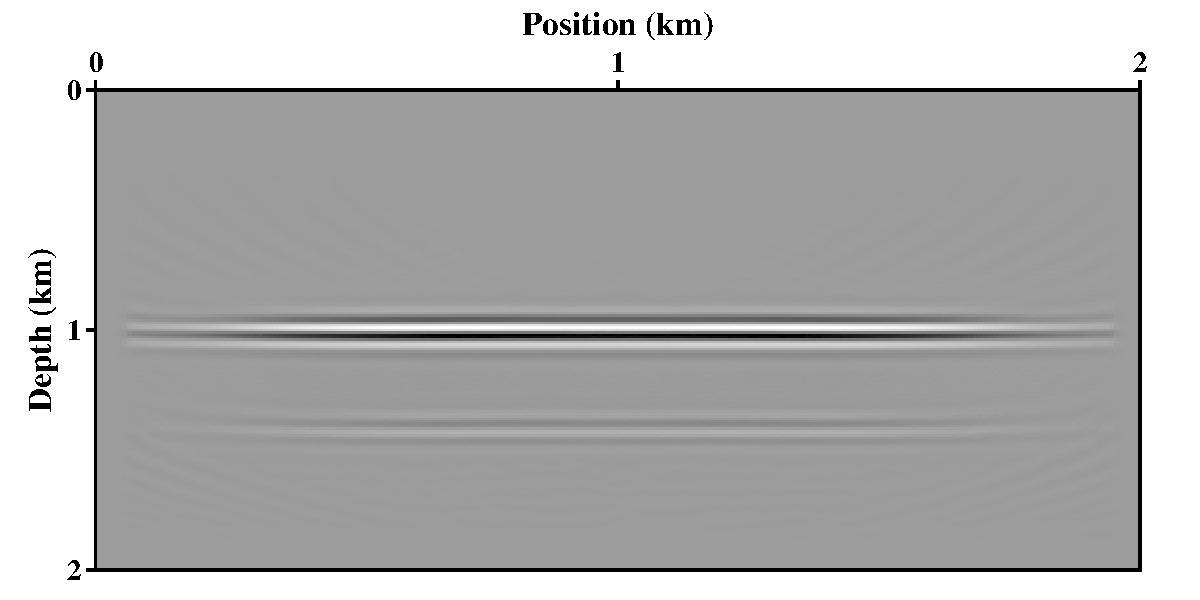
\includegraphics[width=0.5\textwidth]{Figure/chapter04/tradeoff/RTMvpdecomp.pdf}}
   \subfloat[]{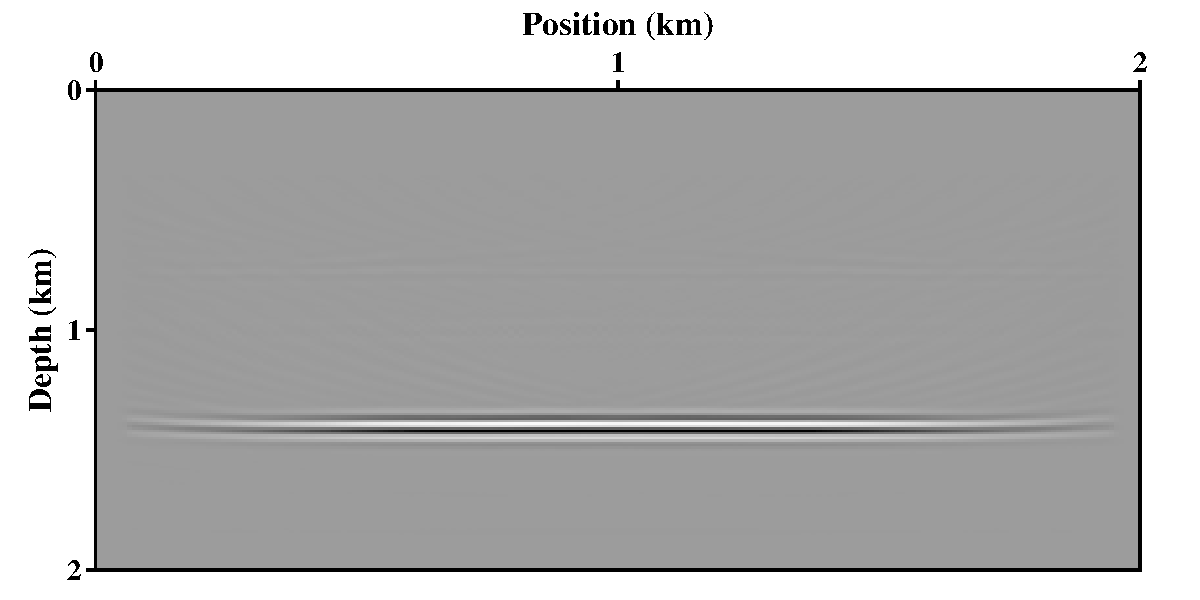
\includegraphics[width=0.5\textwidth]{Figure/chapter04/tradeoff/RTMvsdecomp.pdf}}\\
   \subfloat[]{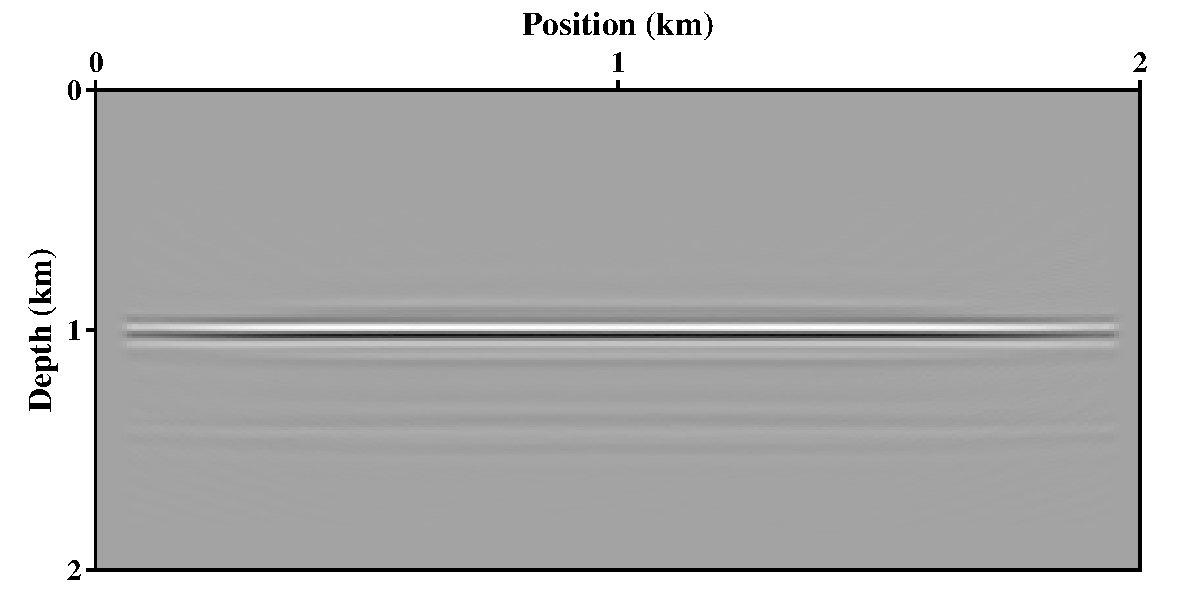
\includegraphics[width=0.5\textwidth]{Figure/chapter04/tradeoff/vpdecomp.pdf}}
   \subfloat[]{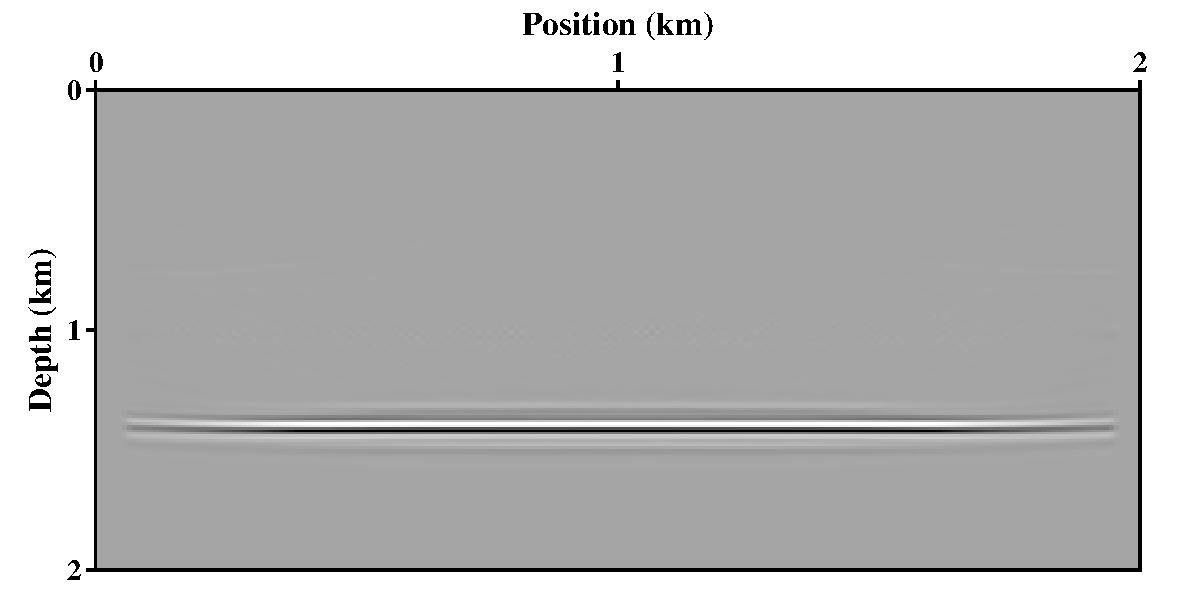
\includegraphics[width=0.5\textwidth]{Figure/chapter04/tradeoff/vsdecomp.pdf}}\\
   \subfloat[]{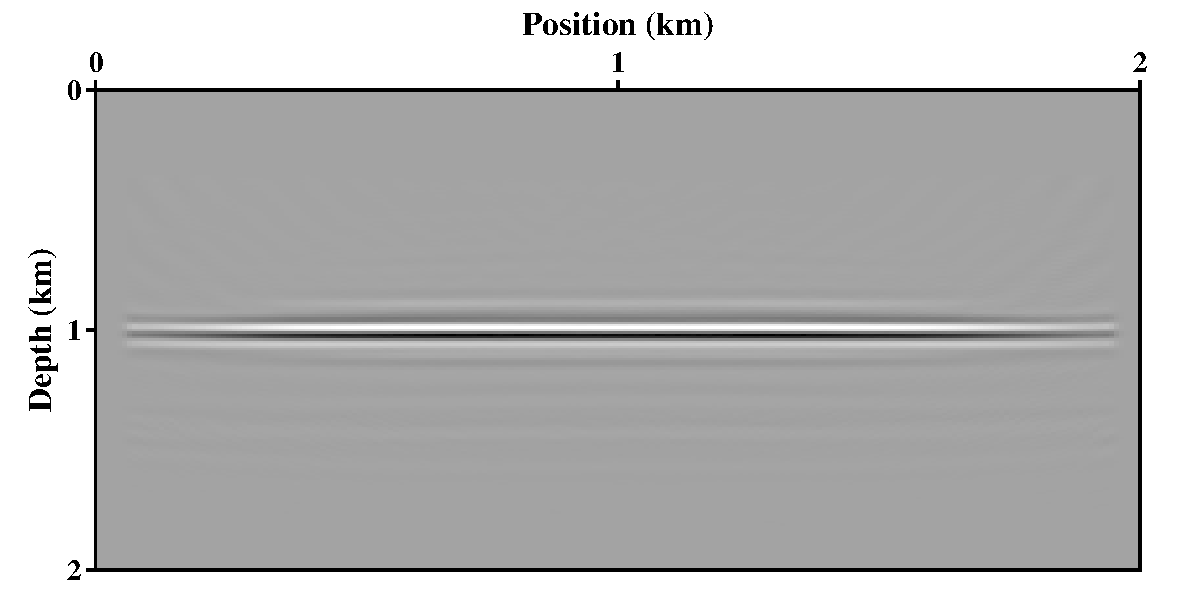
\includegraphics[width=0.5\textwidth]{Figure/chapter04/tradeoff/2ndvpdecomp.pdf}}
   \subfloat[]{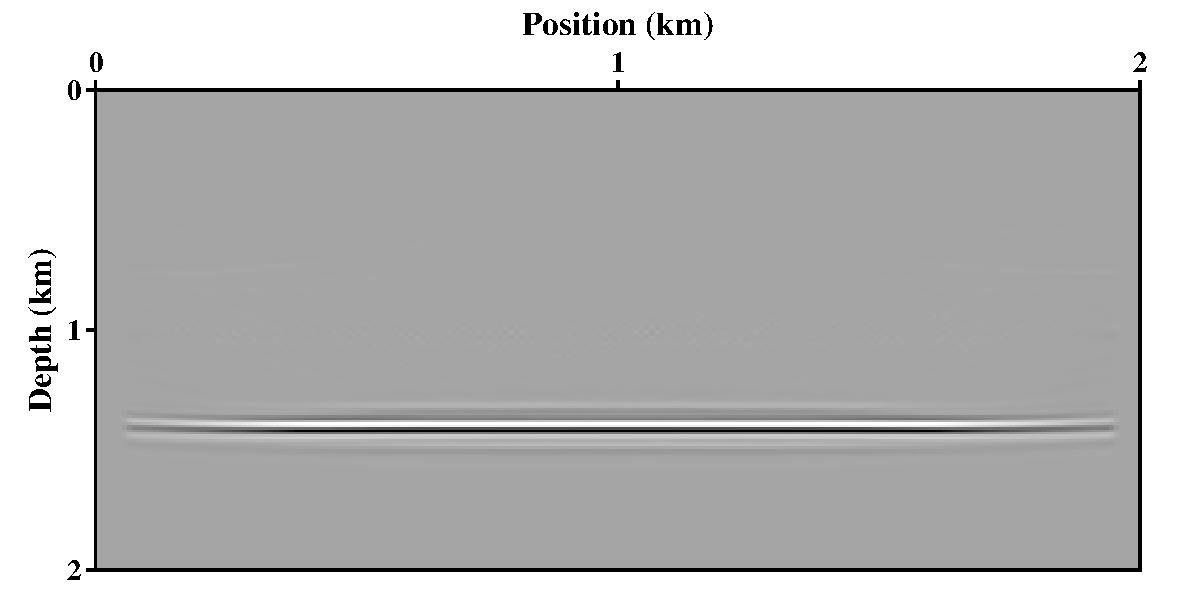
\includegraphics[width=0.5\textwidth]{Figure/chapter04/tradeoff/vsdecomp.pdf}}
   \caption{基于模式解耦的ERTM与ELSRTM结果:左侧为$\delta V_p$,右侧为$\delta V_s$。(a),
   (b) ERTM结果; (c), (d) 采用策略1时ELSRTM结果;(e), (f) 采用策略2时ELSRTM结果。}
   \label{fig:tradeoff_decomp}
\end{figure}
参数耦合同样是ELSRTM中面临的一个挑战。虽然通过最小平方偏移迭代处理,可以一定程度上降低参数间
的串扰,例如Duan et al., 2016\cite{Duan2016};Feng and
Schuster, 2016\cite{Feng2016}。但是这也只能做到压制“脚印”,难以完全消除,
尤其是在$V_p$与$V_s$结构不一致的时候。%而模式解耦的梯度可以很好的帮助降低$V_s$反演中受到的参数耦合干扰。
为了测试参数耦合对ELSRTM的影响,本文
%以及模式解耦的有效性,
选取具有不同结构的$V_p$与$V_s$双层模型(图\ref{fig:tradeoffModel})来进行实验。

这里采用Born正演数据进行双参数同时反演。
由于$V_s$界面也会产生P波反射,
常规RTM结果中$V_p$与$V_s$成像结果存在明显的相互串扰(见图\ref{fig:tradeoff_nodecomp}),而ELSRTM可以压制部分参数耦合效应,
但是难以完全消除,尤其是$\delta V_s$中存在非常明显的$\delta V_p$脚印。
引入模式解耦之后,
首先采用策略1进行反演。
由于采用S波数据来计算$\delta V_s$梯度,
就完全避免了P波对$\delta
V_s$梯度的干扰。根据第二章中所分析的模式解耦帮助压制参数耦合的机制,采用S波反演$V_s$近似于单参数反演,这将
有助于反演的收敛。但是这样并不能在反演初始阶段就对$\delta
V_p$的反演产生明显改善,只能依靠迭代过程中$\delta
V_s$趋近于真值时来消除其所产生的P波数据残差,进而一定程度上提升$\delta V_p$的反演效果。

从ERTM结果上看(图\ref{fig:tradeoff_decomp}a和b),解耦之后的成像结果压制了$\delta V_s$中
$V_p$界面产生的脚印。解耦预条件的ELSRTM得到的$\delta
V_s$已经没有了$V_p$界面的脚印,但是$\delta
V_p$中仍然存在一定的干扰。这是因为在策略1中,初始迭代阶段中$\delta
V_s$更新量不足使得$\delta
V_p$的梯度仍然受到参数耦合的影响。而这个阶段总是能够搜索到较大的更新步长,这就导致在初始阶段的参数耦合效应仍然较为严重,而且主要体现在
$\delta V_p$受到$\delta V_s$的影响。
策略2可以进一步压制这种类型的串扰,因为在$\delta
V_s$反演足够好的时候,$V_s$界面产生的P波数据已经基本匹配,这时再反演$\delta
V_p$,$V_s$界面对$\delta V_p$的影响就会很弱。
当然,反演得到的$\delta V_s$不可能与真值一样,因此数据残差中总会存在少量来自$\delta
V_s$散射的P波。从图\ref{fig:tradeoff_decomp}e和f可以看到,即使采用策略2,$\delta V_p$中仍然会存留非常弱的脚印。


\subsection{Marmousi-II模型}
本节对Marmousi-II模型进行了A和B两种方式的修改,
以进一步测试前文提到的两种反演策略。
模型A:在$V_p$单独加入高速层;模型B:在$V_p$和$V_s$中分别加入不同结构的异常层;
为了降低计算代价,除异常层之外,$V_s$模型都通过固定的泊凇比由$V_p$模型转换而成。
观测系统中60个炮点等间隔地分布在地表。模型空间采样间隔
为10m,时间采样间隔为1ms,模拟时间总长3s,子波主频20Hz。除非特别指明,本节所有数值实验都采用相同的观测系统。
为了对比Born模拟数据与剩余反射数据反演结果的差异,
每个模型都采用两种数据各进行一次ELSRTM。
\begin{figure}[!htb]
   \centering
   \subfloat[]{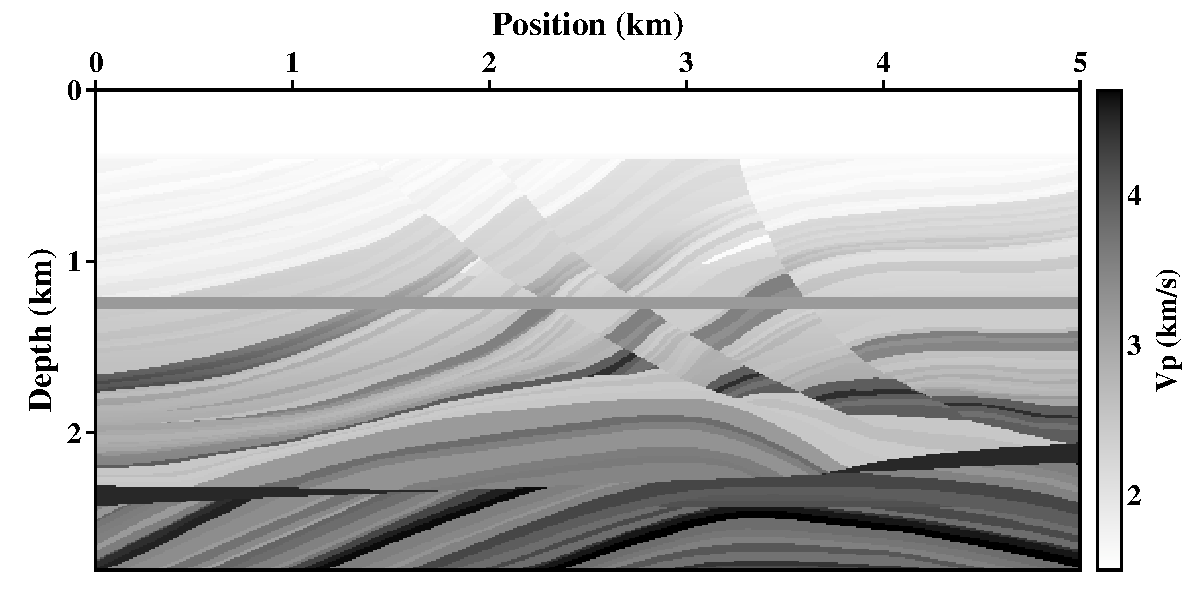
\includegraphics[width=0.5\textwidth]{Figure/chapter04/Marmousi/born/vp.pdf}}
   \subfloat[]{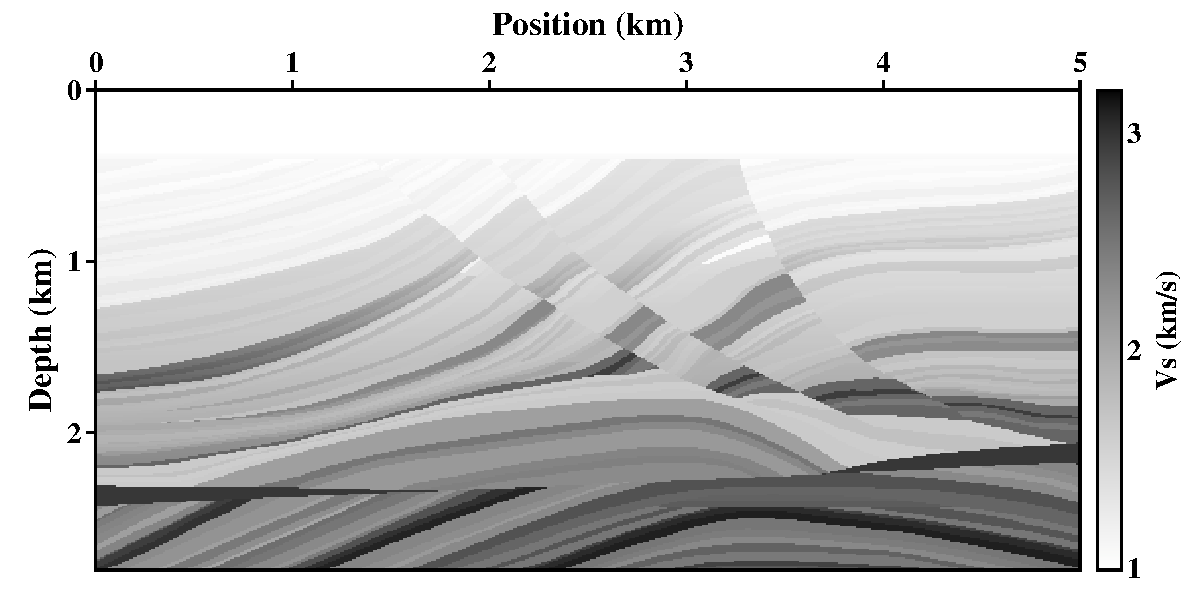
\includegraphics[width=0.5\textwidth]{Figure/chapter04/Marmousi/born/vs.pdf}}\\
   \subfloat[]{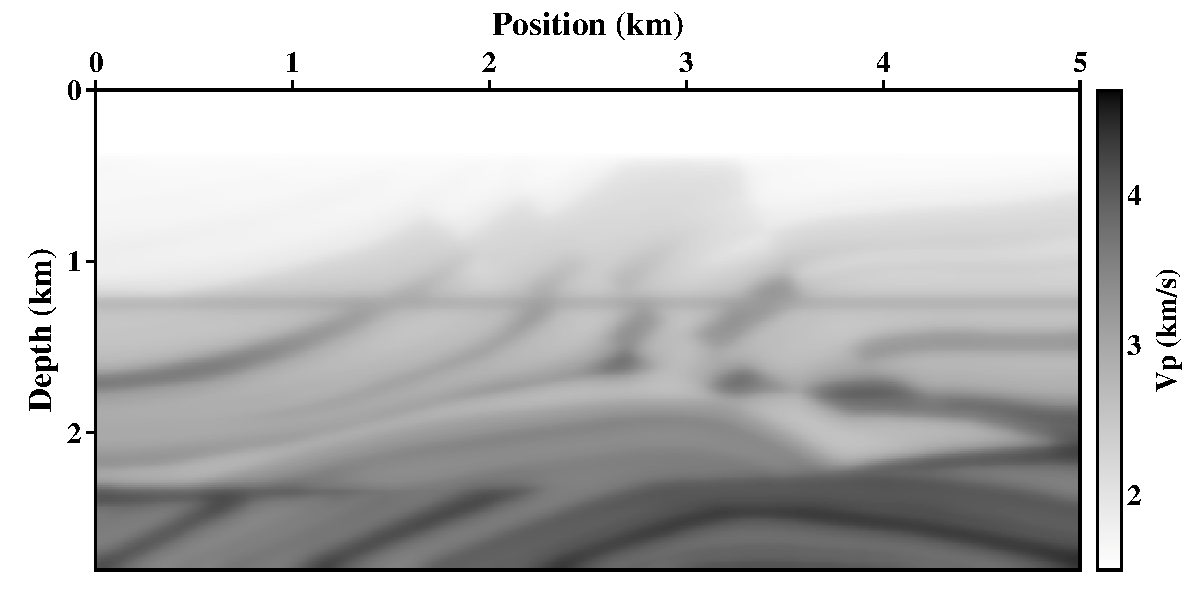
\includegraphics[width=0.5\textwidth]{Figure/chapter04/Marmousi/born/vpsmooth.pdf}}
   \subfloat[]{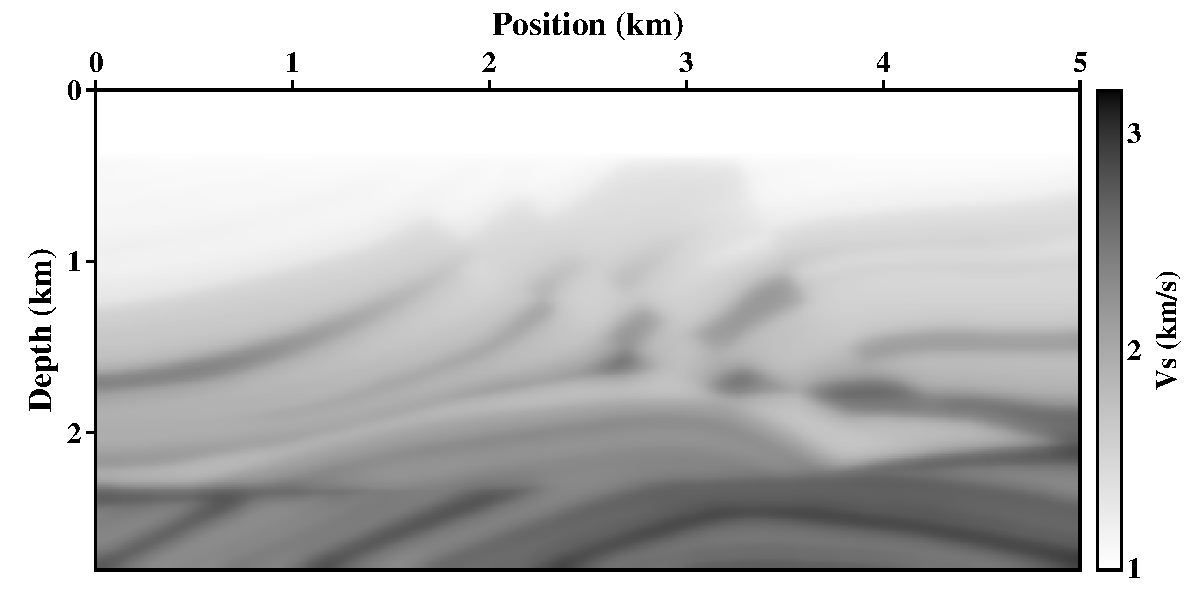
\includegraphics[width=0.5\textwidth]{Figure/chapter04/Marmousi/born/vssmooth.pdf}}
   \caption{A方式修改后的Marmousi-II真实模型与偏移模型:左侧为$V_p$,右侧为$V_s$。第一行为真实模型,第二行为偏移模型。}
   \label{fig:TrueAndInitial_1}
\end{figure}
\begin{figure}[!htb]
   \centering
   \subfloat[]{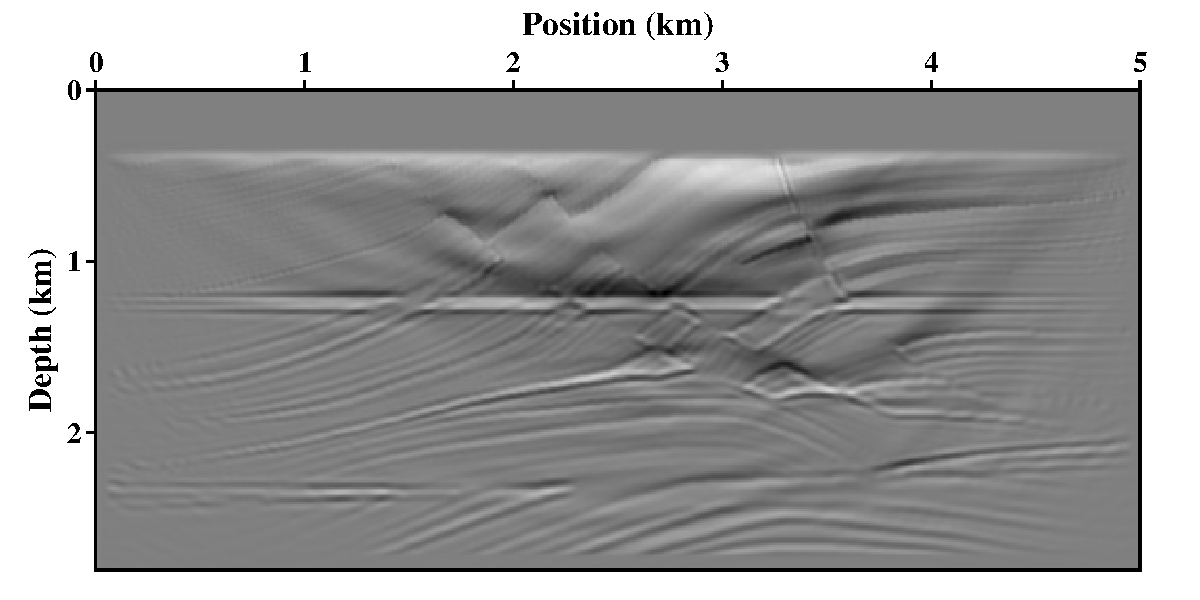
\includegraphics[width=0.5\textwidth]{Figure/chapter04/Marmousi/born/RTMvpnodecomp.pdf}}
   \subfloat[]{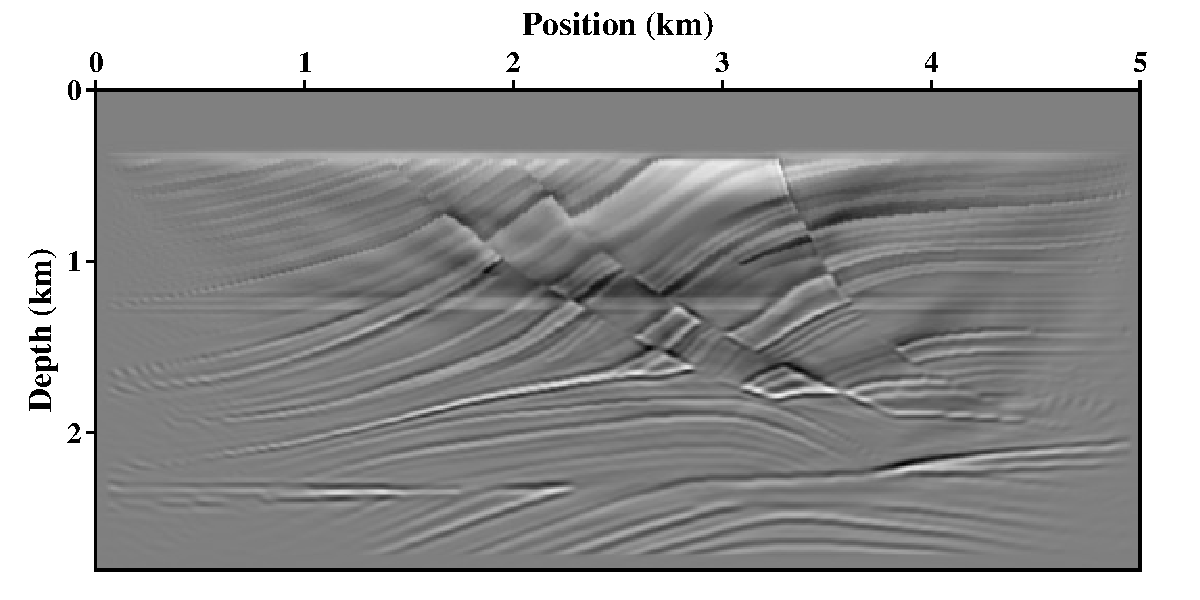
\includegraphics[width=0.5\textwidth]{Figure/chapter04/Marmousi/born/RTMvsnodecomp.pdf}}\\
   \subfloat[]{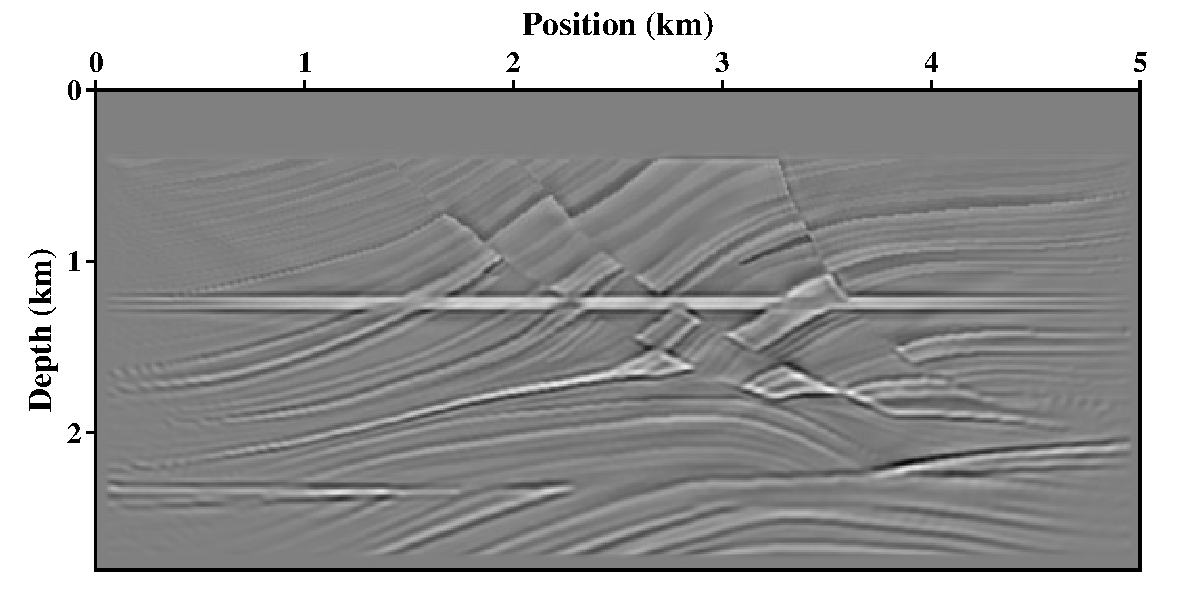
\includegraphics[width=0.5\textwidth]{Figure/chapter04/Marmousi/born/vpnodecomp.pdf}}
   \subfloat[]{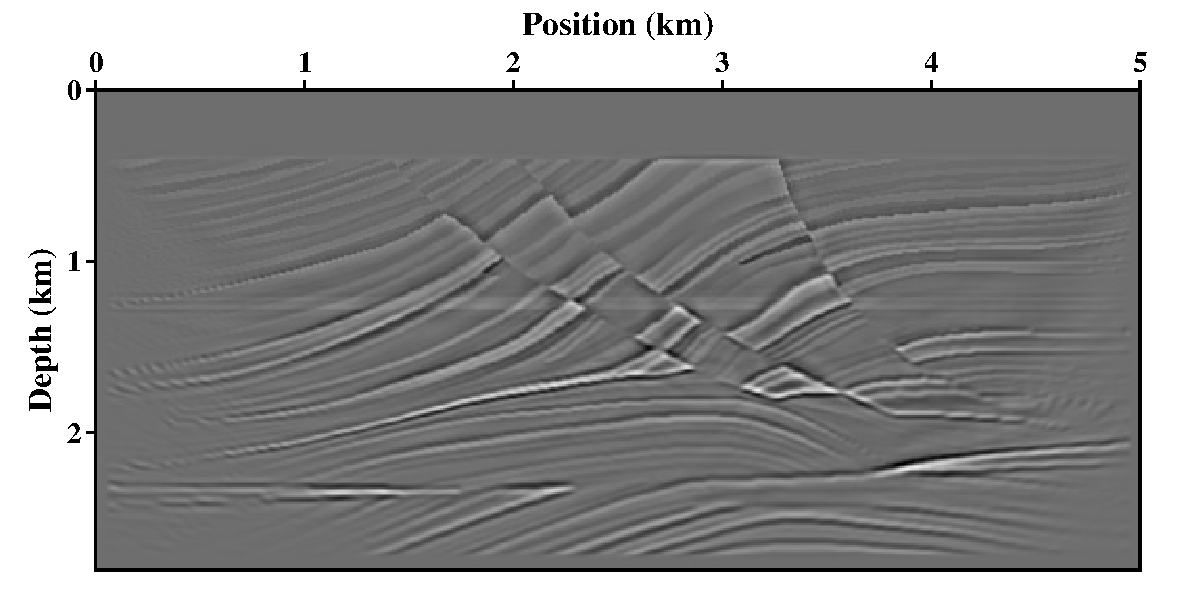
\includegraphics[width=0.5\textwidth]{Figure/chapter04/Marmousi/born/vsnodecomp.pdf}}
   \caption{Born模拟数据常规ERTM与ELSRTM结果(模型A):左侧为$V_p$,右侧为$V_s$。第一行为ERTM结果,第二行为ELSRTM结果。}
   \label{fig:nodecomp_1}
\end{figure}
\begin{figure}[!htb]
   \centering
   \subfloat[]{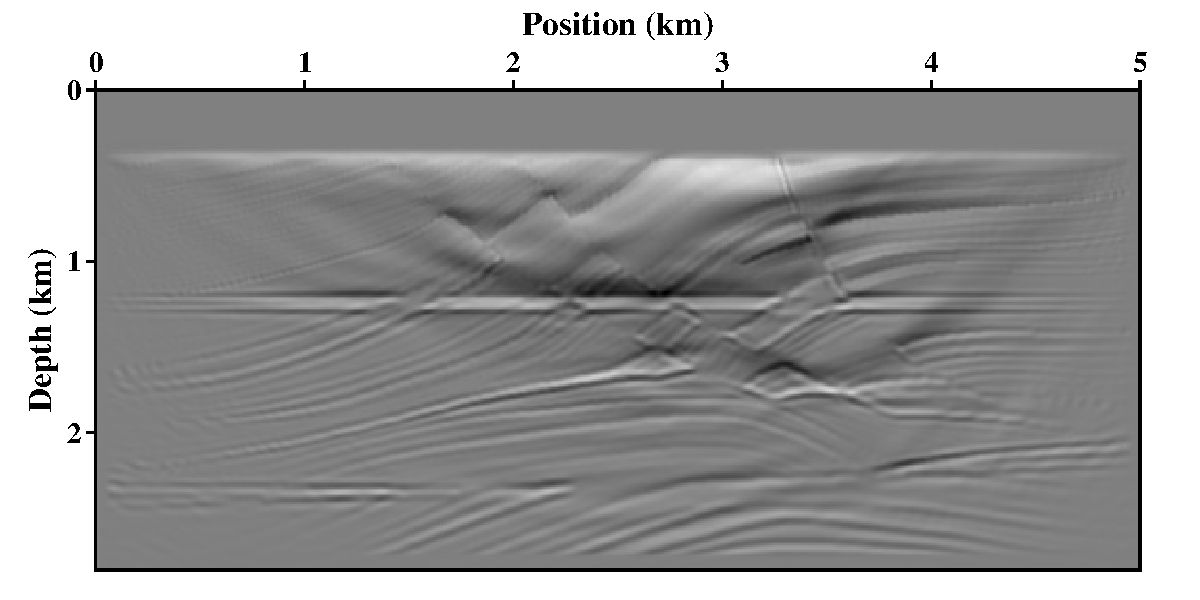
\includegraphics[width=0.5\textwidth]{Figure/chapter04/Marmousi/born/RTMvpdecomp.pdf}}
   \subfloat[]{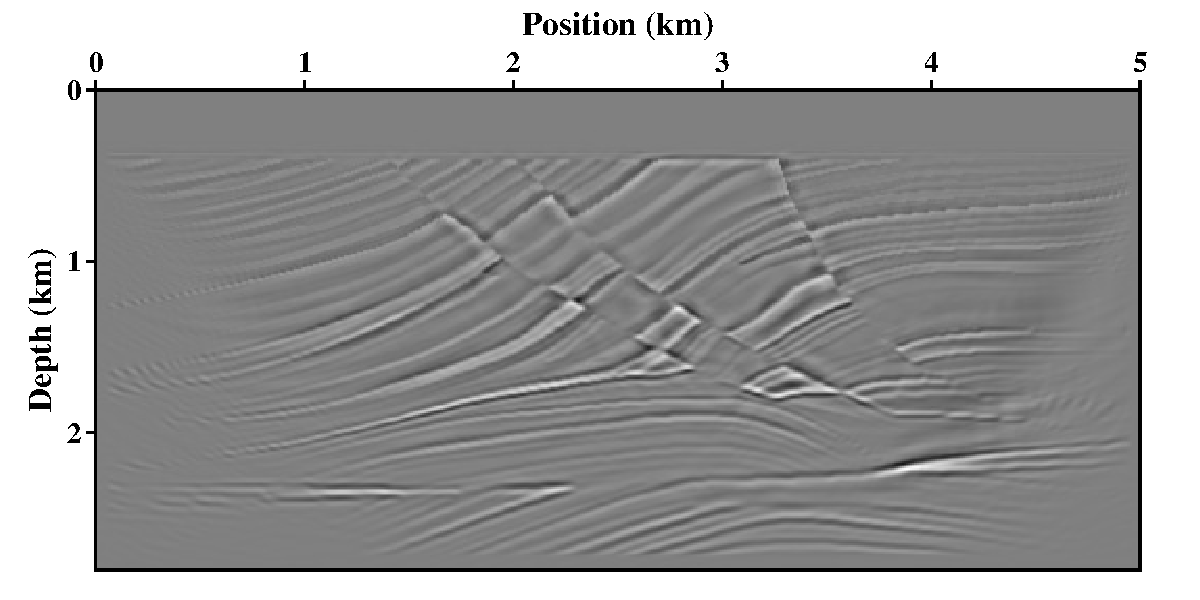
\includegraphics[width=0.5\textwidth]{Figure/chapter04/Marmousi/born/RTMvsdecomp.pdf}}\\
   \subfloat[]{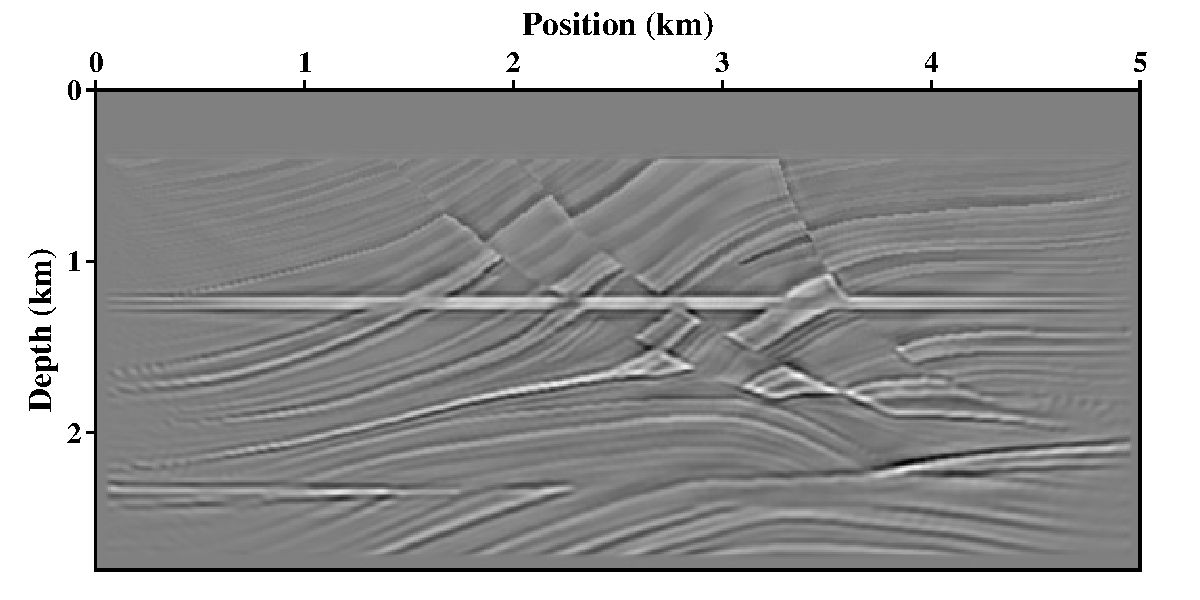
\includegraphics[width=0.5\textwidth]{Figure/chapter04/Marmousi/born/vpdecomp.pdf}}
   \subfloat[]{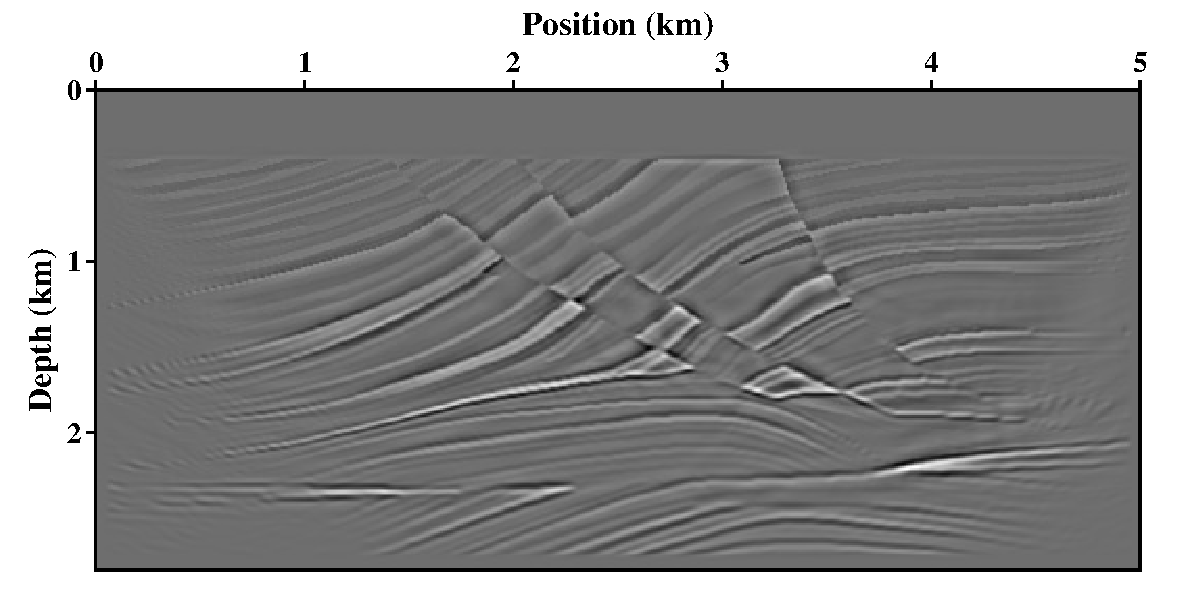
\includegraphics[width=0.5\textwidth]{Figure/chapter04/Marmousi/born/vsdecomp.pdf}}\\
   \caption{Born模拟数据模式解耦ERTM与ELSRTM结果(模型A):左侧为$V_p$,右侧为$V_s$。第一行为ERTM结果,第二行为ELSRTM结果。}
   \label{fig:decomp_1}
\end{figure}

在实验A中,为了突出参数耦合效应,在$V_p$模型中加入了一个高速薄层。这样在常规ELSRTM中,$\delta
V_s$的反演受到的参数耦合影响会非常明显。由于$\delta V_p$较少受到$V_s$结构的影响,因此采用反演策略1,即同时反演$\delta
V_p$与$\delta
V_s$。首先采用Born模拟数据进行实验。如图\ref{fig:nodecomp_1}所示,常规ERTM
的成像剖面中可以看到低频噪音的干扰。由于参数耦合,$\delta
V_s$中还存在$V_p$结构的脚印。在经过ELSRTM之后,低频噪音被压制,
整个成像剖面能量更加均衡。$\delta V_s$中的参数耦合效应虽然被部分压制了,但是仍然可以看到残留的脚印。

然后将模式解耦预条件处理加入到梯度计算中,成像与反演结果如图\ref{fig:decomp_1}所示。ERTM中$\delta
V_p$仍然存在低频噪音,而$\delta
V_s$中的低频噪音已经很大程度上被压制。这说明$\delta
V_s$中的低频噪音主要是P波路径所产生,所以在经过模式解耦压制了反传波场中的P波成分后,ERTM就可以获得无低频噪音的$\delta
V_s$。与此同时,其中来自$V_p$结构的脚印也被完全压制。在经过ELSRTM之后,低频噪音被进一步地压制,而且深部与浅部的能量也更加均衡。
最终获得了较高分辨率的$\delta V_p$与$\delta V_s$结果。
\begin{figure}[!htb]
   \centering
   \subfloat[]{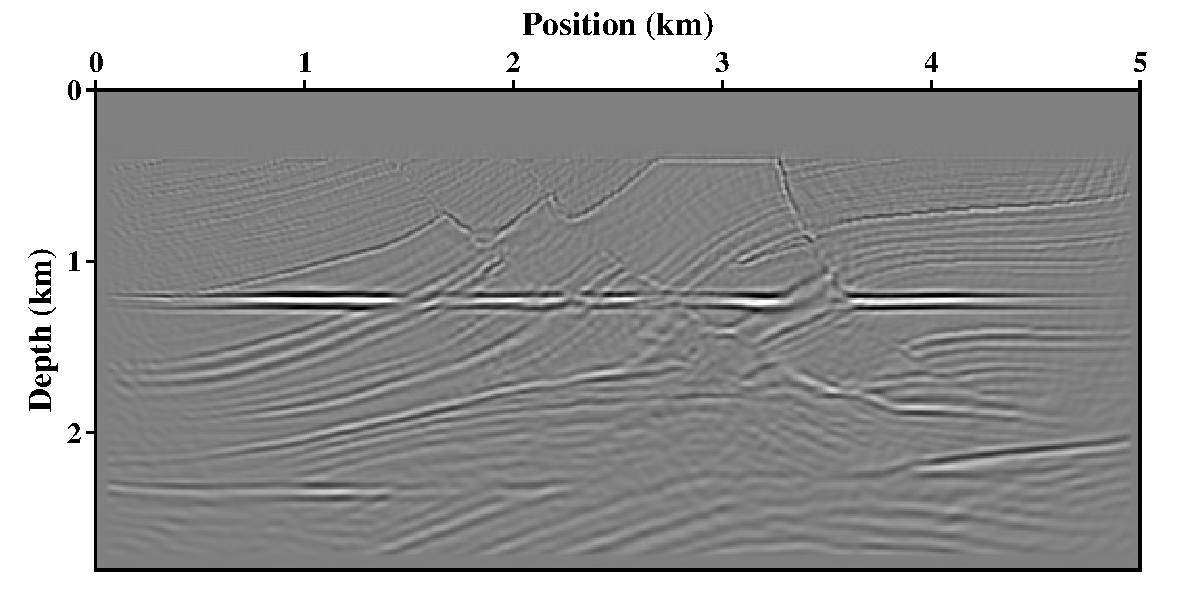
\includegraphics[width=0.5\textwidth]{Figure/chapter04/Marmousi/reflection/RTMvpnodecomp.pdf}}
   \subfloat[]{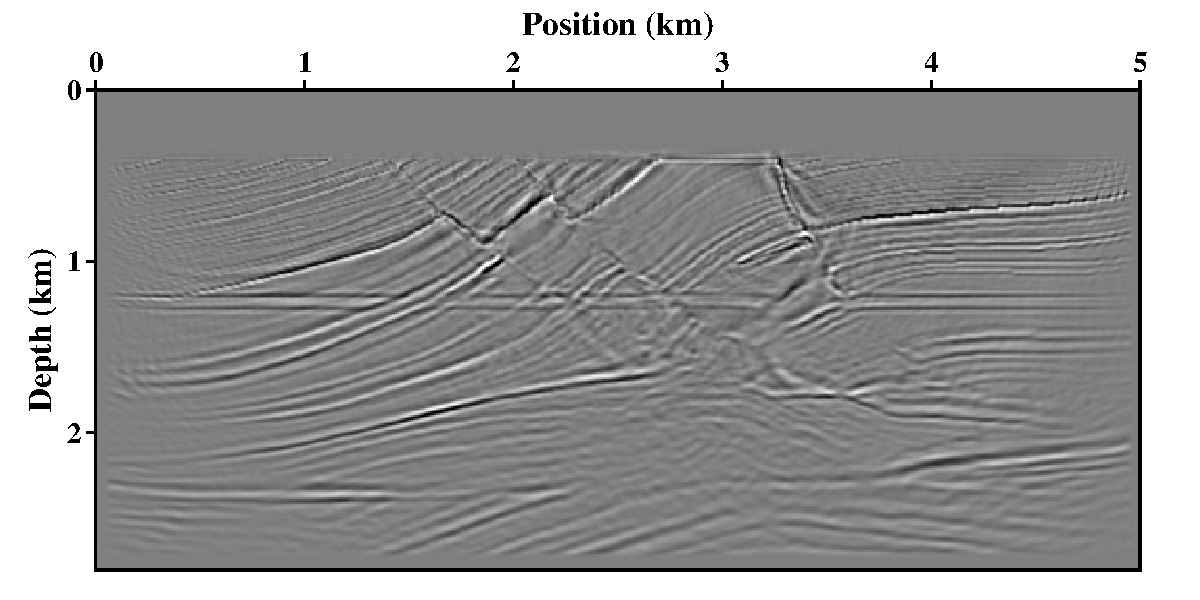
\includegraphics[width=0.5\textwidth]{Figure/chapter04/Marmousi/reflection/RTMvsnodecomp.pdf}}\\
   \subfloat[]{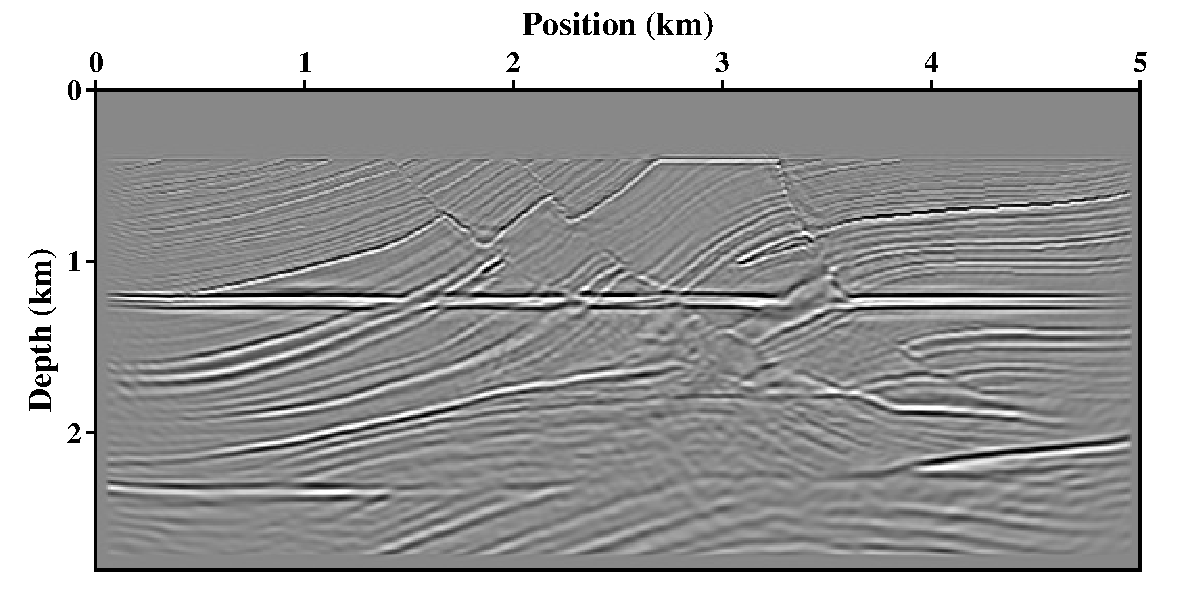
\includegraphics[width=0.5\textwidth]{Figure/chapter04/Marmousi/reflection/vpnodecomp.pdf}}
   \subfloat[]{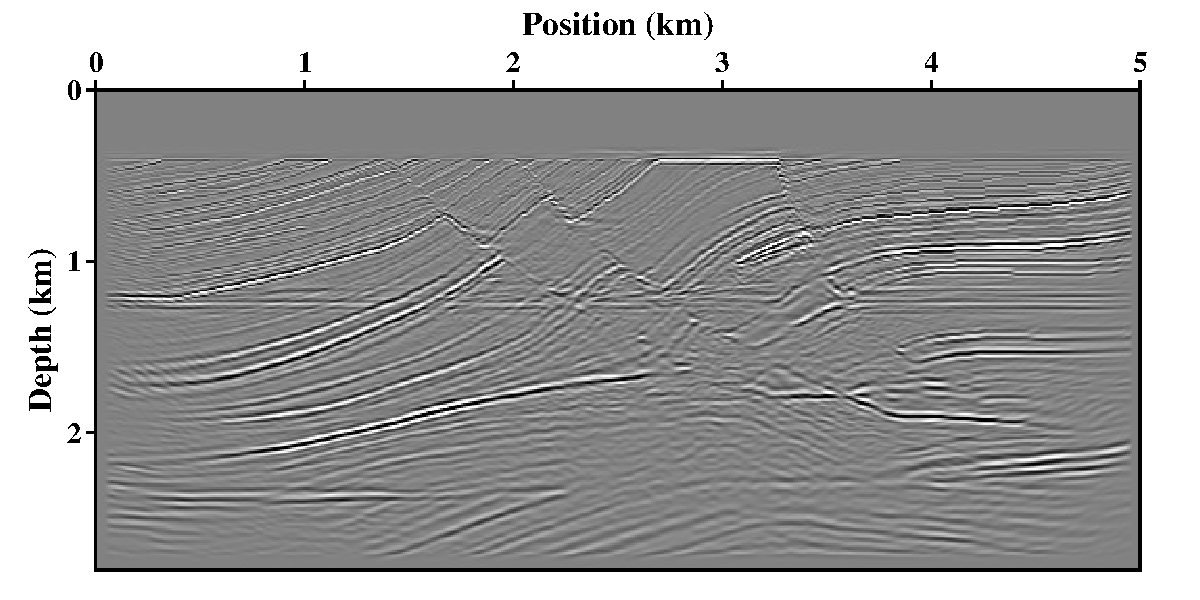
\includegraphics[width=0.5\textwidth]{Figure/chapter04/Marmousi/reflection/vsnodecomp.pdf}}
   \caption{剩余反射数据常规ERTM与ELSRTM结果(模型A):左侧为$V_p$,右侧为$V_s$。第一行为ERTM结果,第二行为ELSRTM结果。}
   \label{fig:node_1_refl}
\end{figure}

虽然理论上Born模拟数据与剩余反射数据相差不多,但这只是考虑一次散射的情况。在复杂介质中,多次散射很强时利用反射数据进行LSRTM就会遇到挑战。
接下来,将采用剩余反射数据测试算法。反射数据中的直达波会带来很大的干扰,因此在进行实验时先根据走时对直达波进行切除。
常规ERTM成像与ELSRTM反演结果如图\ref{fig:node_1_refl}所示,由于切除了直达波,ERTM结果已基本不受低频噪音干扰,
但是模型深部成像能量不均衡,且存在参数耦合问题。在中间断层区域,多次散射
效应很明显,引起许多串扰的假象。经过ELSRTM之后,深部的能量获得了较好的补偿,分辨率也得到了提高,但是参数耦合导致$\delta
V_s$结果中来自$\delta V_p$的脚印难以被彻底压制。
\begin{figure}[!hbt]
   \centering
   \subfloat[]{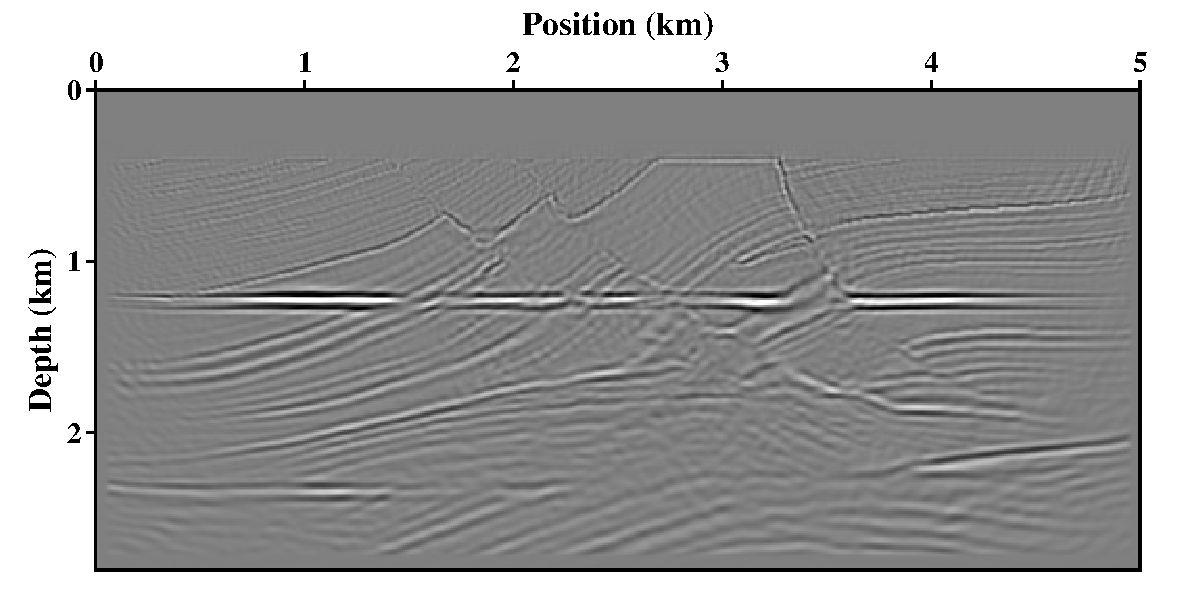
\includegraphics[width=0.5\textwidth]{Figure/chapter04/Marmousi/reflection/RTMvpdecomp.pdf}}
   \subfloat[]{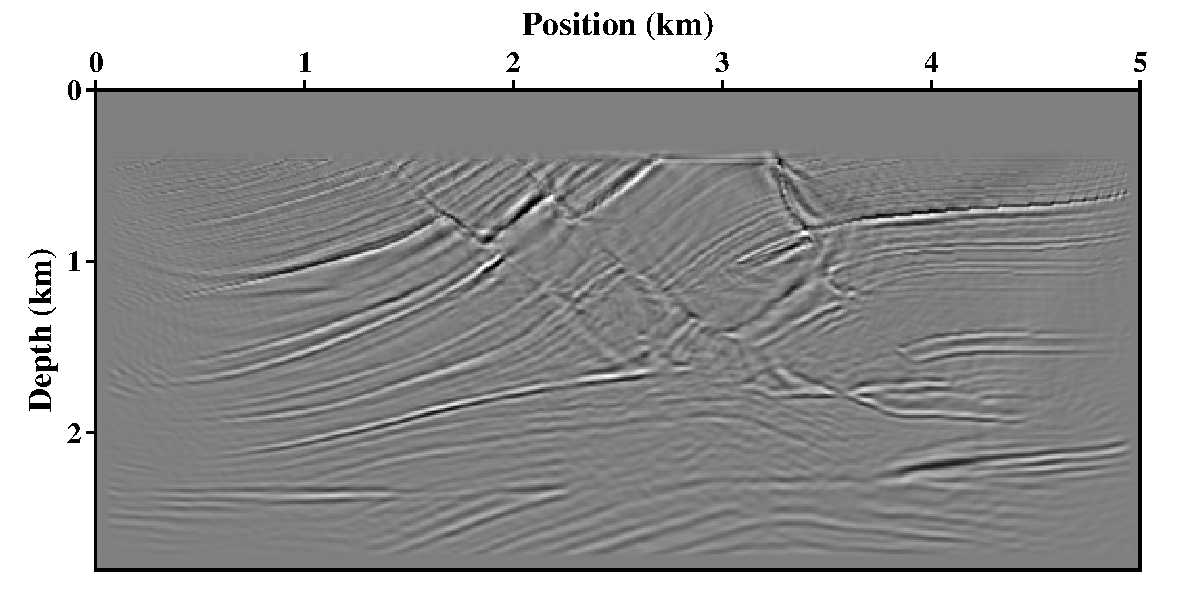
\includegraphics[width=0.5\textwidth]{Figure/chapter04/Marmousi/reflection/RTMvsdecomp.pdf}}\\
   \subfloat[]{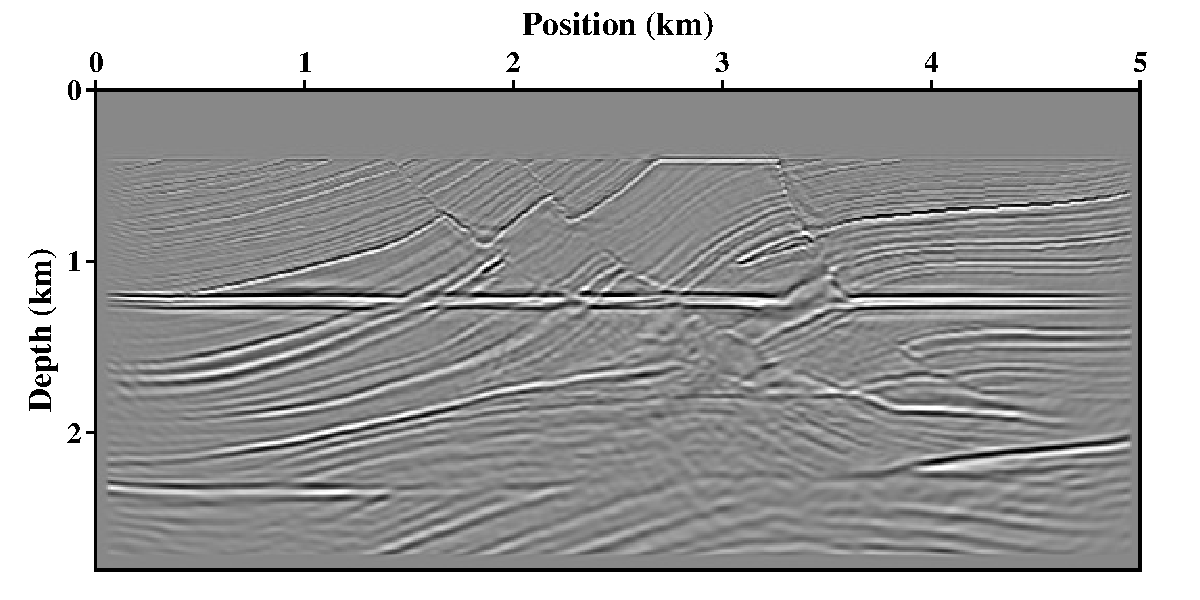
\includegraphics[width=0.5\textwidth]{Figure/chapter04/Marmousi/reflection/vpdecomp.pdf}}
   \subfloat[]{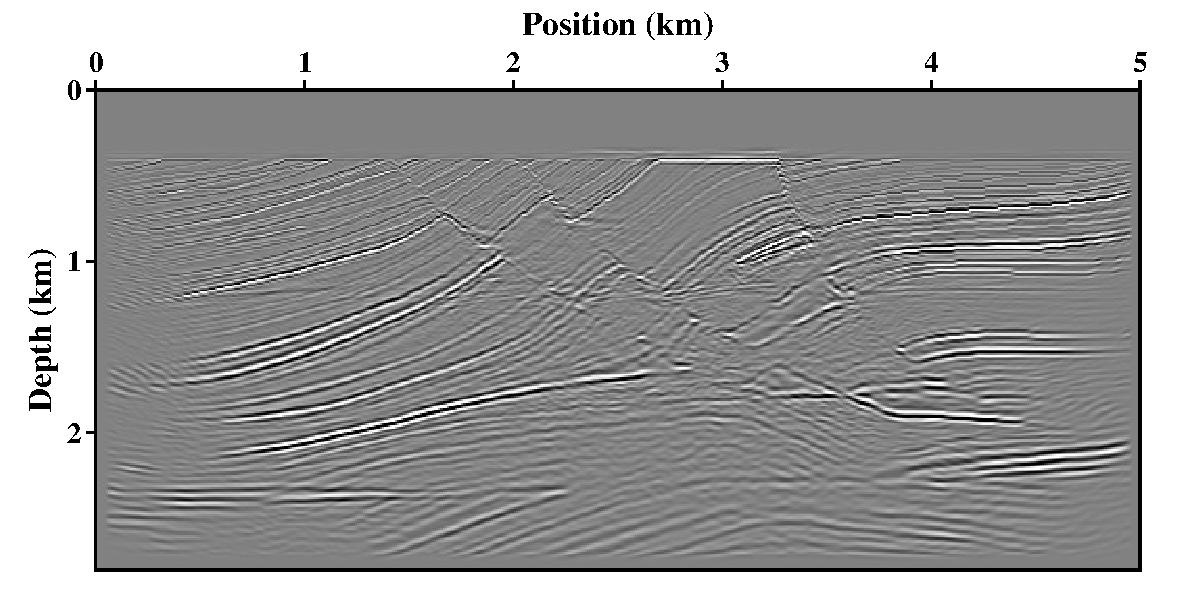
\includegraphics[width=0.5\textwidth]{Figure/chapter04/Marmousi/reflection/vsdecomp.pdf}}
   \caption{剩余反射数据模式解耦ERTM与ELSRTM结果(模型A):左侧为$V_p$,右侧为$V_s$。第一行为ERTM结果,第二行为ELSRTM结果。}
   \label{fig:de_1_refl}
\end{figure}

在引入模式解耦之后(图\ref{fig:de_1_refl}),可以看到ERTM获得的$\delta
V_s$结果中的脚印已经被压制。再经过ELSRTM之后,成像分辨率得到了提高,深部区域的能量也经过补偿获得了均衡。
从结果上看Born模拟数据要比剩余反射数据的反演效果好,这是因为:第一,Born模拟数据的正演与反演过程完全匹配;
第二,剩余反射数据中存在多次散射效应。不管怎样,采用模式解耦的梯度预条件能够在ELSRTM中进一步压制参数耦合效应。
\begin{figure}[!hbt]
   \centering
   \subfloat[]{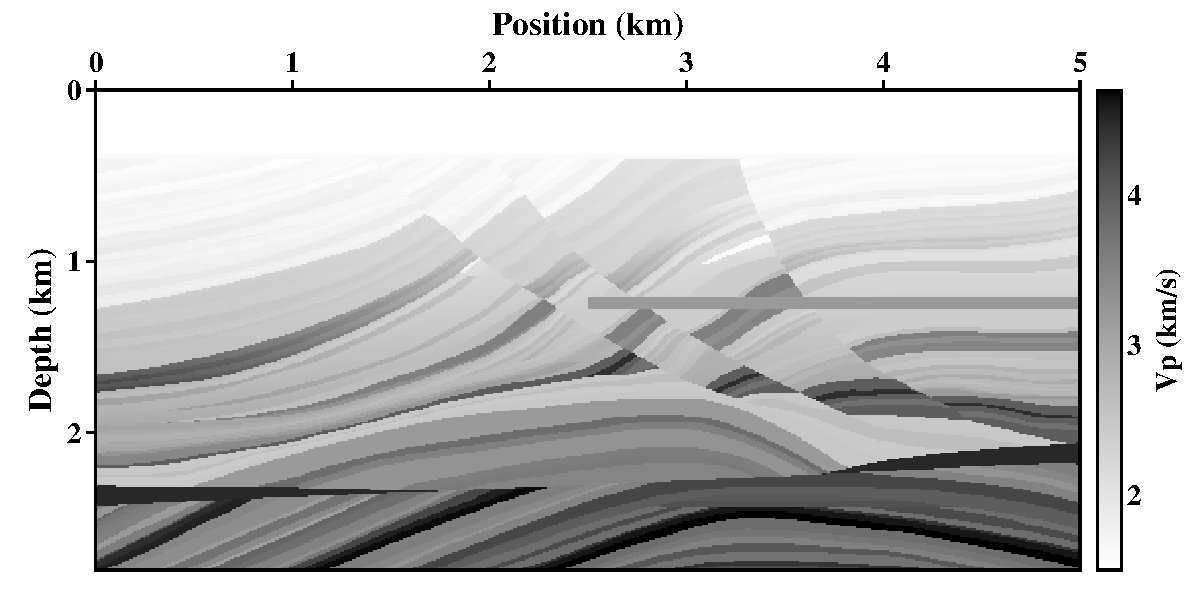
\includegraphics[width=0.5\textwidth]{Figure/chapter04/Marmousi/Vsborn/vp.pdf}}
   \subfloat[]{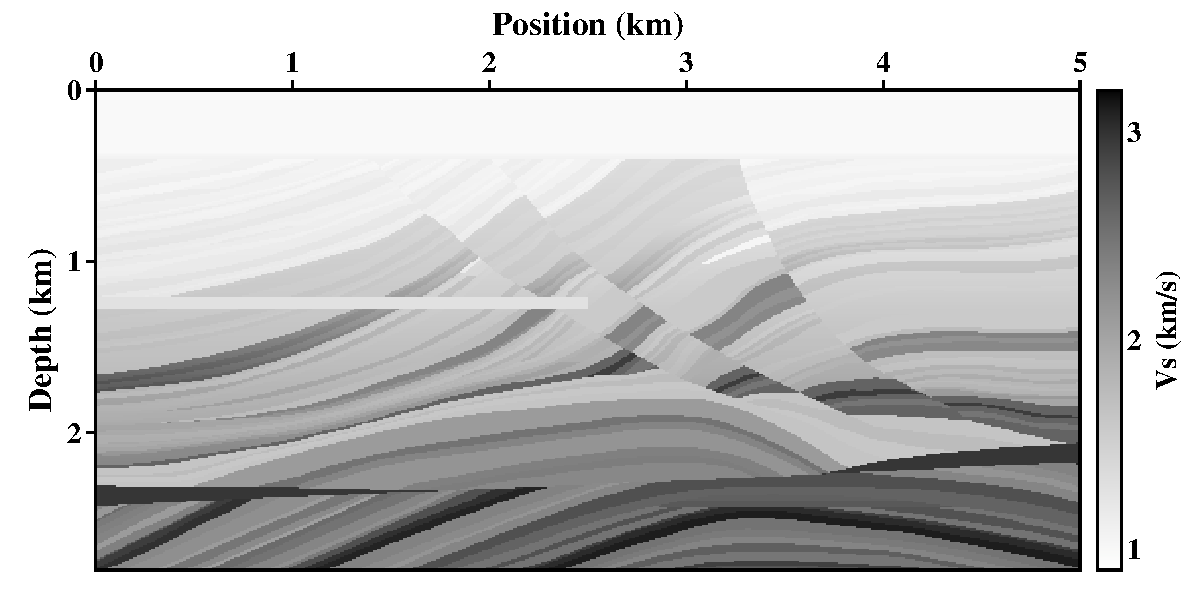
\includegraphics[width=0.5\textwidth]{Figure/chapter04/Marmousi/Vsborn/vs.pdf}}\\
   \subfloat[]{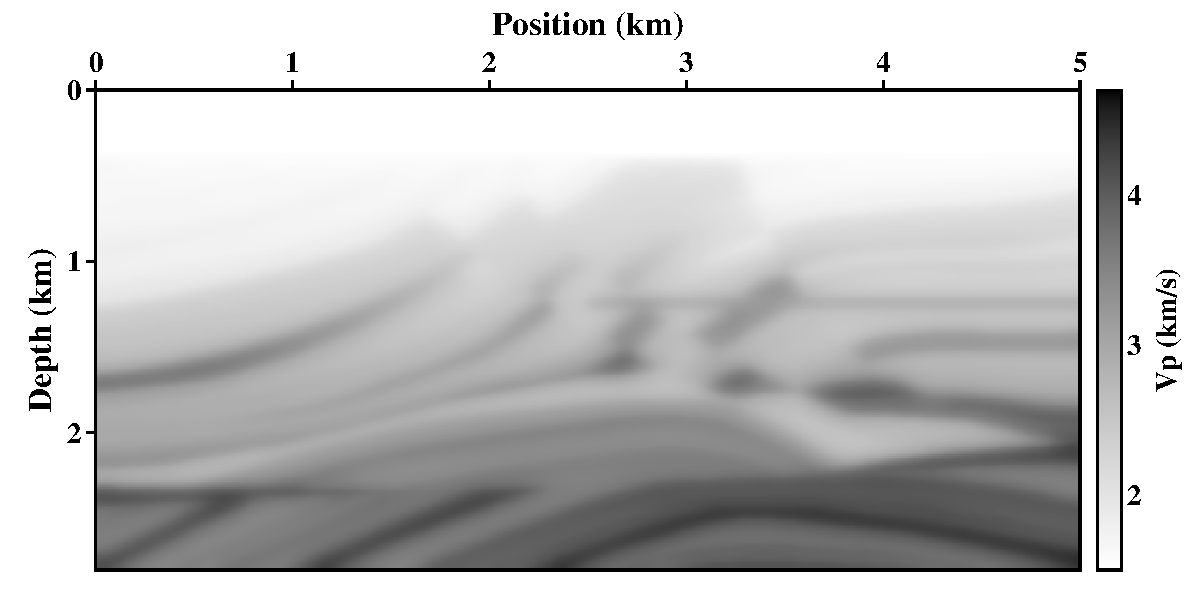
\includegraphics[width=0.5\textwidth]{Figure/chapter04/Marmousi/Vsborn/vpsmooth.pdf}}
   \subfloat[]{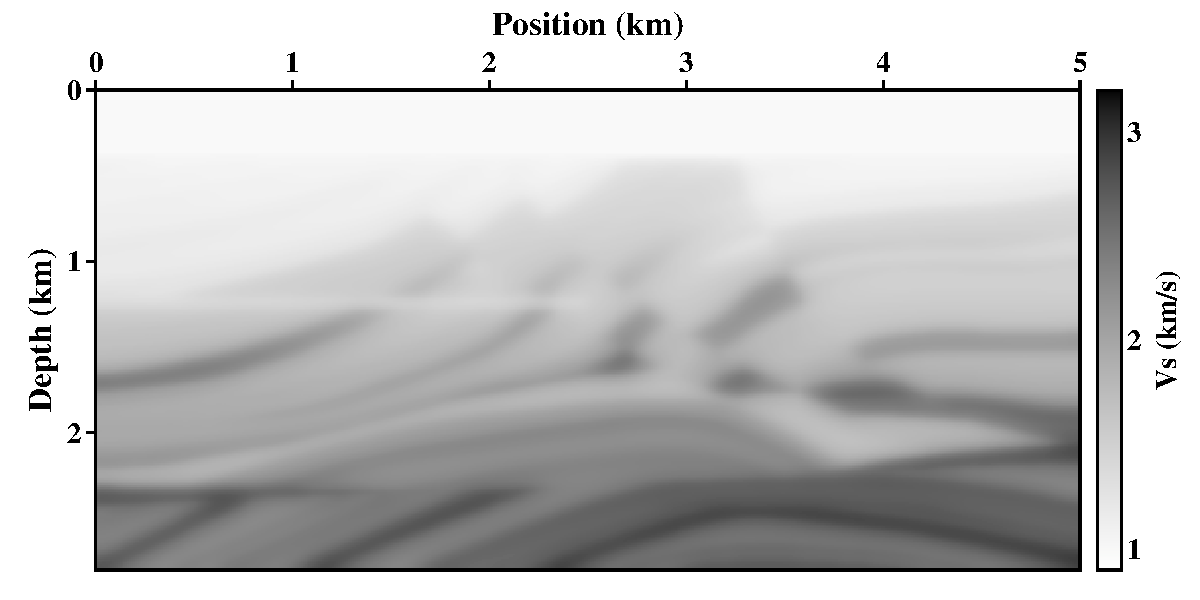
\includegraphics[width=0.5\textwidth]{Figure/chapter04/Marmousi/Vsborn/vssmooth.pdf}}
   \caption{B方式修改后的Marmousi-II真实模型与偏移模型:左侧为$V_p$,右侧为$V_s$。第一行为真实模型,第二行为偏移模型。}
   \label{fig:TrueAndInitial_2}
\end{figure}

\begin{figure}[!hbt]
   \centering
   \subfloat[]{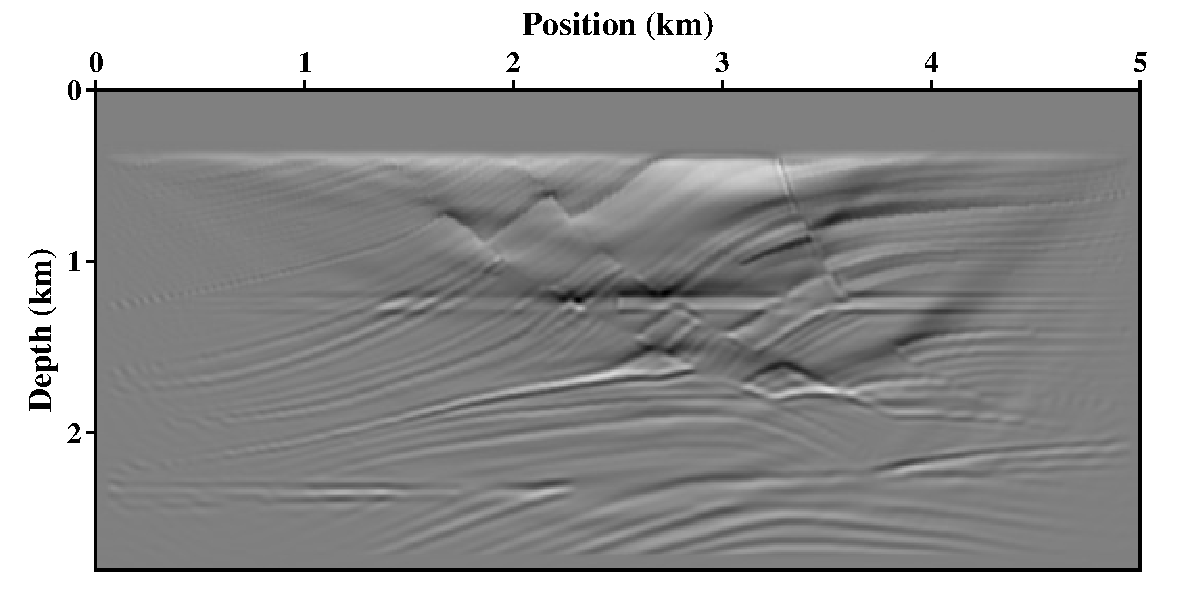
\includegraphics[width=0.5\textwidth]{Figure/chapter04/Marmousi/Vsborn/RTMvpnodecomp.pdf}}
   \subfloat[]{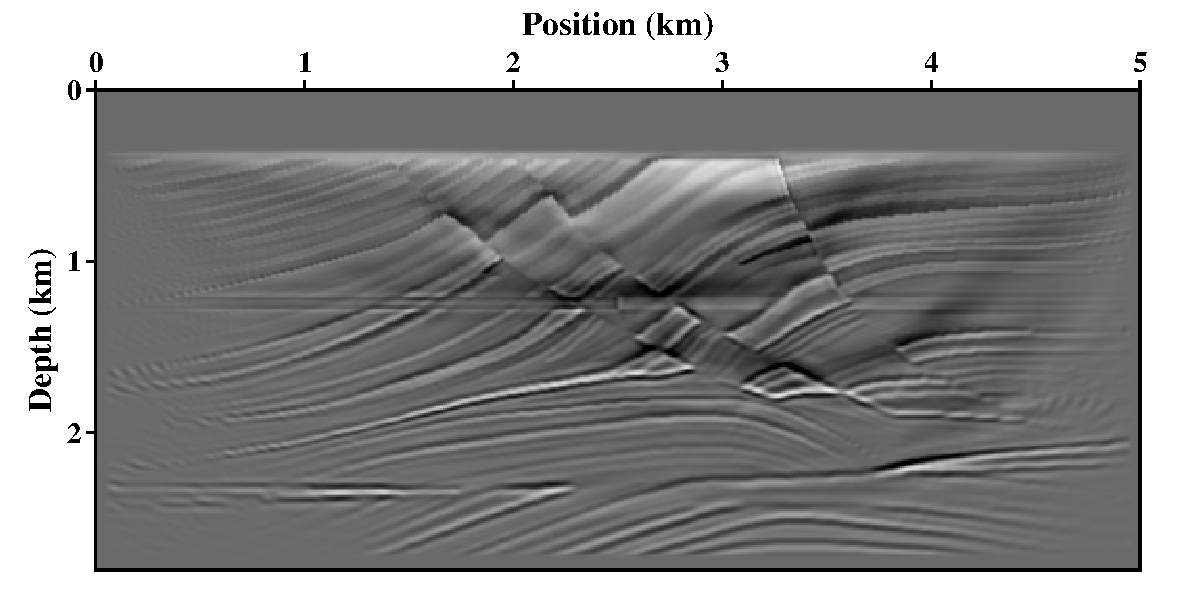
\includegraphics[width=0.5\textwidth]{Figure/chapter04/Marmousi/Vsborn/RTMvsnodecomp.pdf}}\\
   \subfloat[]{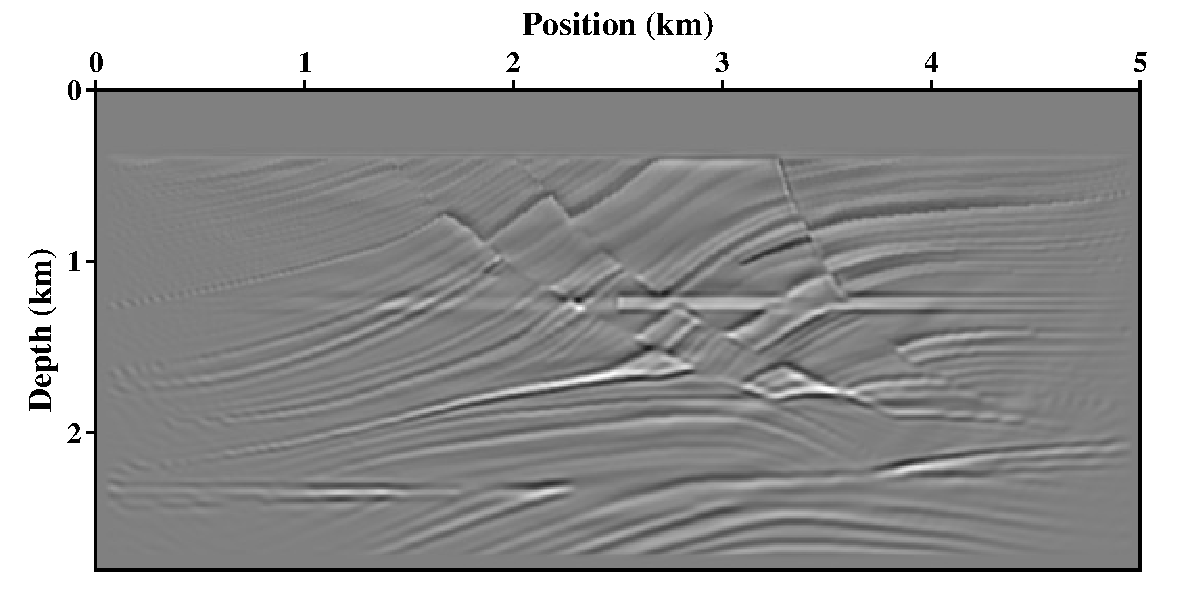
\includegraphics[width=0.5\textwidth]{Figure/chapter04/Marmousi/Vsborn/vpnodecomp.pdf}}
   \subfloat[]{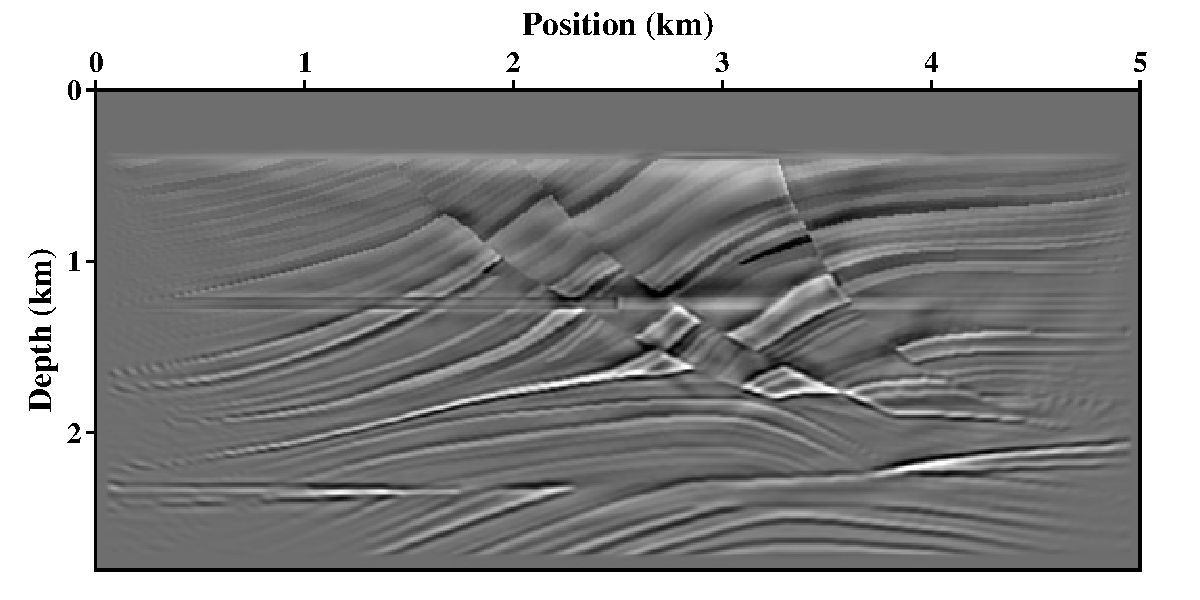
\includegraphics[width=0.5\textwidth]{Figure/chapter04/Marmousi/Vsborn/vsnodecomp.pdf}}
   \caption{Born模拟数据常规ERTM与ELSRTM结果(模型B):左侧为$V_p$,右侧为$V_s$。第一行为ERTM结果,第二行为ELSRTM结果。}
   \label{fig:nodecomp_2}
\end{figure}
\begin{figure}[!hbt]
   \centering
   \subfloat[]{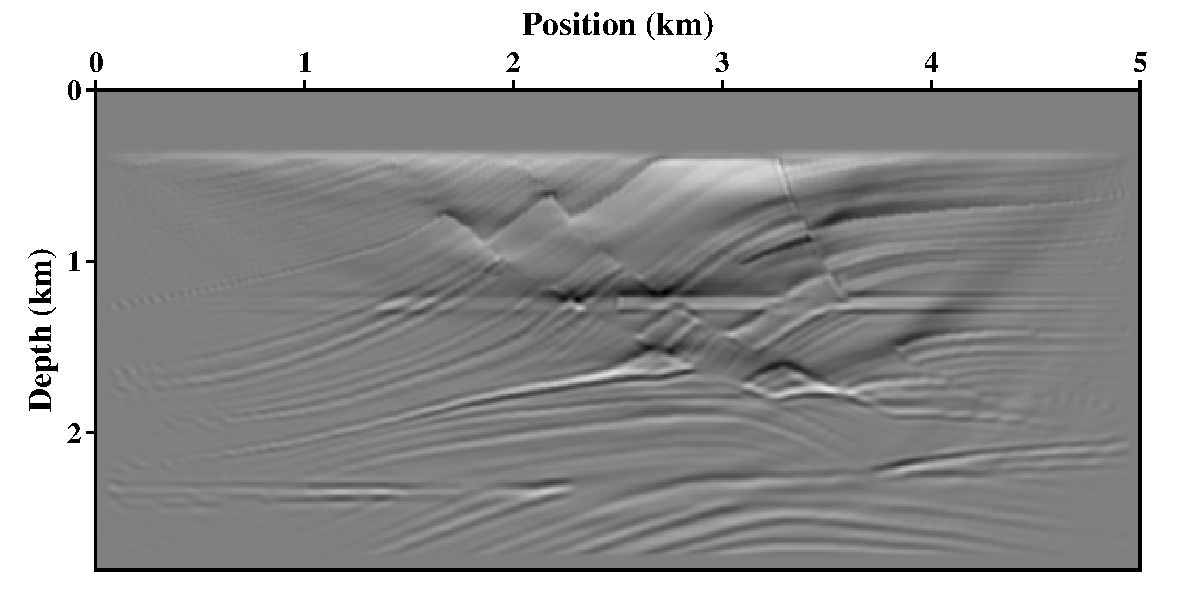
\includegraphics[width=0.5\textwidth]{Figure/chapter04/Marmousi/Vsborn/RTMvpdecomp.pdf}}
   \subfloat[]{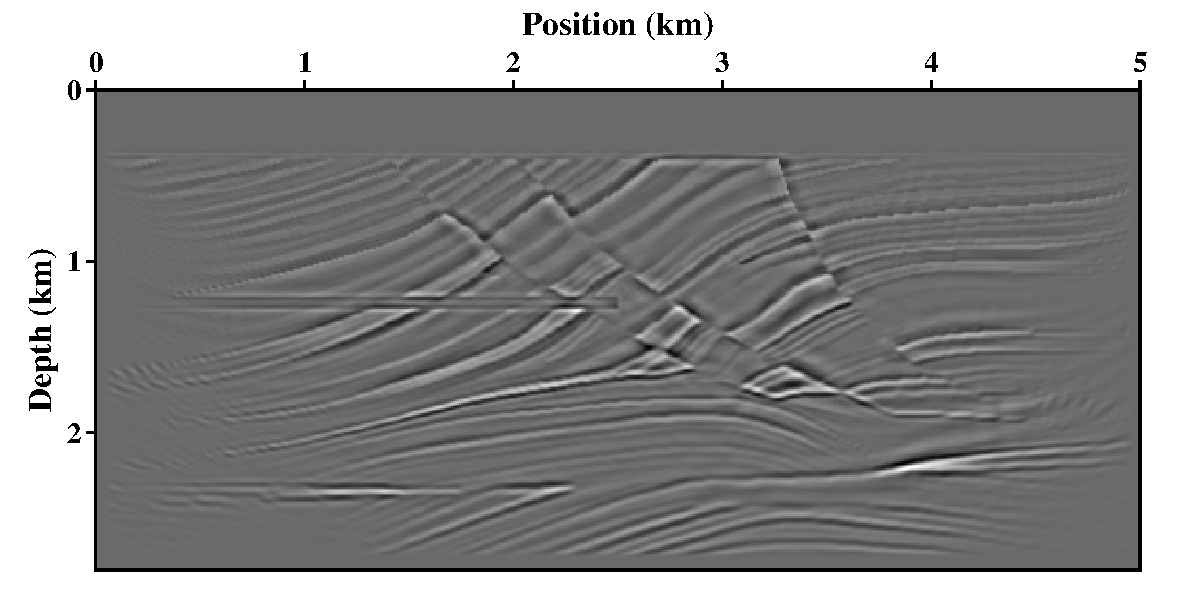
\includegraphics[width=0.5\textwidth]{Figure/chapter04/Marmousi/Vsborn/RTMvsdecomp.pdf}}\\
   \subfloat[]{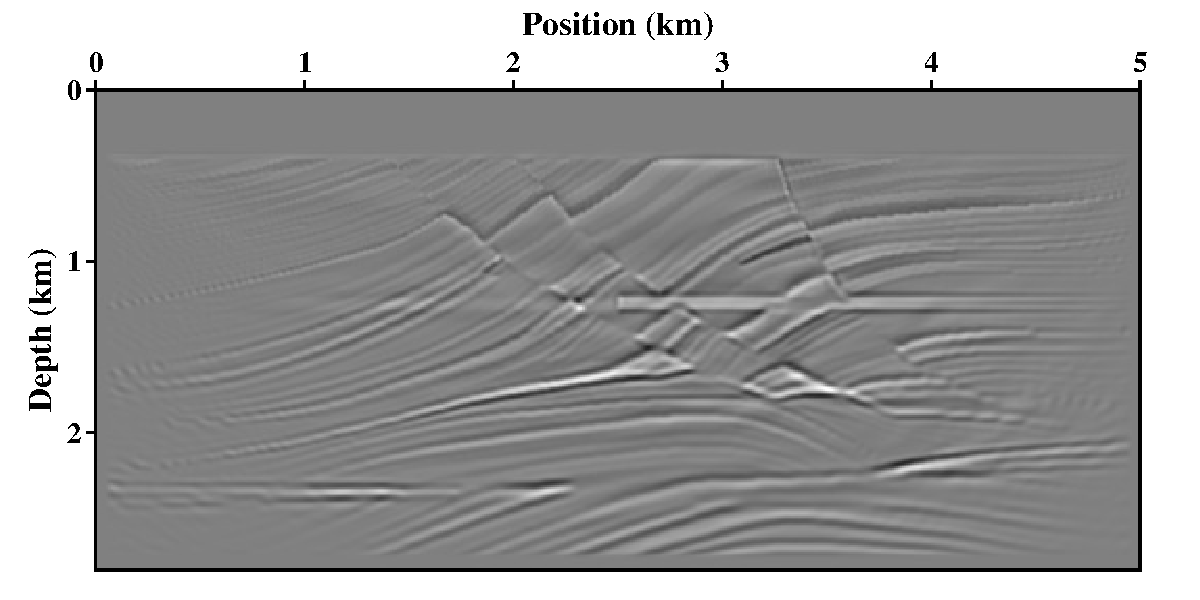
\includegraphics[width=0.5\textwidth]{Figure/chapter04/Marmousi/Vsborn/vpdecomp.pdf}}
   \subfloat[]{\includegraphics[width=0.5\textwidth]{Figure/chapter04/Marmousi/Vsborn/vsdecomp.pdf}}
   \caption{Born模拟数据模式解耦ERTM与ELSRTM结果(模型B):左侧为$V_p$,右侧为$V_s$。第一行为ERTM结果,第二行为ELSRTM结果。}
   \label{fig:decomp_2}
\end{figure}
在实验B中,为了进一步突出参数耦合效应,在$V_p$和$V_s$模型中分别加入不同的速度异常结构(图\ref{fig:TrueAndInitial_2})。
这样参数耦合会在两个参数反演结果中产生比较严重的脚印。这是在实际数据很容易遇到的情况。
此时如果考虑同时反演(策略1),
ELSRTM的非线性程度会增高。Born模拟数据的常规ELSRTM图像中,$\delta
V_s$甚至还存在低频噪音。一个可能的原因就是右侧受到参数耦合的影响,导致P波没有或者错误的匹配。
采用模式解耦的梯度之后,不论ERTM还是ELSRTM,都消除了$\delta
V_s$中的参数耦合,但是$\delta
V_p$中仍然存在部分的耦合脚印。这是由于$\delta
V_s$的反演没有完全收敛到真值,导致数据中总有来自$\delta V_s$的残余P波。
这部分假象很难被完全消除掉。并且对于反射数据,正反演过程并不完全匹配,
所以这种假象在同时反演中难以被消除,这就需要考虑策略2。

\begin{figure}[!htb]
   \centering
   \subfloat[]{\includegraphics[width=0.5\textwidth]{Figure/chapter04/Marmousi/Vsreflection/RTMvpnodecomp.pdf}}
   \subfloat[]{\includegraphics[width=0.5\textwidth]{Figure/chapter04/Marmousi/Vsreflection/RTMvsnodecomp.pdf}}\\
   \subfloat[]{\includegraphics[width=0.5\textwidth]{Figure/chapter04/Marmousi/Vsreflection/vpnodecomp.pdf}}
   \subfloat[]{\includegraphics[width=0.5\textwidth]{Figure/chapter04/Marmousi/Vsreflection/vsnodecomp.pdf}}
   \caption{剩余反射数据常规ERTM与ELSRTM结果,左侧为$V_p$,右侧为$V_s$。第一行为ERTM结果,第二行为ELSRTM结果。}
   \label{fig:nodecomp_2_refl}
\end{figure}
\begin{figure}[!htb]
   \centering
   \subfloat[]{\includegraphics[width=0.5\textwidth]{Figure/chapter04/Marmousi/Vsreflection/RTMvpdecomp.pdf}}
   \subfloat[]{\includegraphics[width=0.5\textwidth]{Figure/chapter04/Marmousi/Vsreflection/RTMvsdecomp.pdf}}\\
   \subfloat[]{\includegraphics[width=0.5\textwidth]{Figure/chapter04/Marmousi/Vsreflection/vpdecomp.pdf}}
   \subfloat[]{\includegraphics[width=0.5\textwidth]{Figure/chapter04/Marmousi/Vsreflection/vsdecomp.pdf}}\\
   \caption{剩余反射数据模式解耦ERTM与ELSRTM结果,左侧为$V_p$,右侧为$V_s$。第一行为ERTM结果,第二行为ELSRTM结果。}
   \label{fig:decomp_2_refl}
\end{figure}
\begin{figure}[!htb]
   \centering
   \subfloat[]{\includegraphics[width=0.5\textwidth]{Figure/chapter04/Marmousi/Vsreflection/vpdecomp.pdf}}
   \subfloat[]{\includegraphics[width=0.5\textwidth]{Figure/chapter04/Marmousi/Vsreflection/firstvs2ndvpdecomp.pdf}}
   \caption{
   模式解耦下策略1与策略2所得到的$\delta
   V_p$反演结果对比。(a) 策略1,(b) 策略2。}
   \label{fig:final_comparison_2}
\end{figure}
下面将在剩余反射数据实验中验证策略2的有效性。
同样对合成数据中的直达波进行了切除。
首先进行双参数同时反演(策略1)。如图\ref{fig:nodecomp_2_refl}所示,常规ERTM与ELSRTM的结果与前面实验结果类似,ELSRTM可以改善成像质量,提高分辨率,
并部分压制参数耦合效应。在采用模式解耦之后,ERTM以及ELSRTM结果中(图\ref{fig:decomp_2_refl})$\delta
V_s$的假象有所压制,但是$\delta
V_p$中的假象仍然存在。然后采用策略2来进行反演。
先用解耦预条件的方式反演好$\delta V_s$,再来反演$\delta
V_p$。由于第一阶段中相当于只利用S波残差进行梯度计算(交叉项近似),因此策略2的$\delta
V_s$反演结果与图\ref{fig:decomp_2}d中采用策略1获得的$\delta V_s$结果基本一致,
这里由于篇幅限制就不再展示。
而采用两步法反演的$\delta
V_p$如图\ref{fig:final_comparison_2}b所示,相比策略1获得的$\delta
V_p$(图\ref{fig:final_comparison_2}a),可以看到左侧速度结构异常区域的干扰被进一步压制。
但是由于$\delta V_s$反演并未完全消除其产生的P波残差,最终反演结果中仍然存在少量的干扰。
\section{本章小结}
ELSRTM可视为线性的EFWI过程,同样会受到参数耦合的影响。虽然该过程
可以提高成像分辨率,但是无法完全压制$\delta V_p$与$\delta V_s$的串扰。模式解耦的预条件处理可以非常有效地压制$\delta
V_s$中来自$\delta V_p$的串扰。
在$\delta V_p$受参数耦合影响较弱时,采用模式解耦预条件梯度进行双参数同时反演可以快速地获得高分辨率的$\delta
V_s$与$\delta V_p$。而在$\delta V_p$受参数耦合影响较强时,通过模式解耦先反演$\delta V_s$后反演$\delta
V_p$,能够进一步压制$\delta V_p$中来自$\delta V_s$的串扰。

在ELSRTM过程中,由于Born模拟数据与反射数据存在差异,直接匹配反射数据会导致界面参数扰动的过估计。
匹配剩余反射数据则可以更好地近似Born散射过程。此外,在模型复杂区域,反射数据中包含有多次散射波,它们会给基于Born近似的ELSRTM带来较多的干扰。

